\documentclass[10pt,a4paper]{report}
\usepackage[utf8]{inputenc}
\usepackage[T1]{fontenc}
\usepackage{lmodern}
\usepackage[margin=2cm,top=2.5cm,bottom=2.5cm]{geometry}
\usepackage{amsmath,amssymb}
\usepackage{booktabs}
\usepackage{longtable}
\usepackage{tabularx}
\usepackage{multirow}
\usepackage{array}
\usepackage{enumitem}
\usepackage[table]{xcolor}
\usepackage{colortbl}
\usepackage{tikz}
\usetikzlibrary{shapes.geometric,arrows.meta,positioning,fit,calc,backgrounds,decorations.pathreplacing}
\usepackage{tcolorbox}
\tcbuselibrary{skins,breakable}
\usepackage{listings}
\usepackage{fancyhdr}
\usepackage{titlesec}
\usepackage[colorlinks=true,linkcolor=blue!70!black,citecolor=blue!70!black,urlcolor=blue!70!black]{hyperref}

% Page styling
\pagestyle{fancy}
\fancyhf{}
\fancyhead[L]{\small\textsf{\textbf{Technical Audit Report} --- Guardian Layer (\texttt{guardian\_layer})}}
\fancyhead[R]{\small\textsf{\thepage}}
\fancyfoot[L]{\small\textsf{Classification: \textbf{CONFIDENTIAL / INTERNAL} | Revision 1.0}}
\fancyfoot[R]{\small\textsf{Ref: NIST SP 800-207 / 800-57 / ISO 27001}}
\renewcommand{\headrulewidth}{0.5pt}
\renewcommand{\footrulewidth}{0.5pt}

% Title formats
\titleformat{\chapter}[display]
  {\normalfont\sffamily\huge\bfseries\color{blue!80!black}}
  {\chaptertitlename\ \thechapter}{14pt}{\Huge}
\titlespacing*{\chapter}{0pt}{-20pt}{20pt}

% Listings styling
\lstset{
  basicstyle=\ttfamily\scriptsize,
  breaklines=true,
  frame=single,
  backgroundcolor=\color{gray!5},
  keywordstyle=\color{blue!80!black}\bfseries,
  commentstyle=\color{green!50!black}\itshape,
  stringstyle=\color{red!70!black},
  showstringspaces=false,
  numbers=none,
  tabsize=2
}

% TColorBox Styles
\newtcolorbox{findingbox}[4]{
  enhanced,
  breakable,
  colback=white,
  colframe=#3,
  coltitle=white,
  fonttitle=\bfseries\sffamily,
  title={Finding #1: #2 \hfill [Severity: #4]},
  boxrule=1.2pt,
  arc=2mm,
  boxsep=2mm
}

\newtcolorbox{adrbox}[3]{
  enhanced,
  breakable,
  colback=white,
  colframe=blue!70!black,
  coltitle=white,
  fonttitle=\bfseries\sffamily,
  title={Architecture Decision Record #1: #2 \hfill [Verdict: #3]},
  boxrule=1.2pt,
  arc=2mm,
  boxsep=2mm
}

\newtcolorbox{callout}[2]{
  enhanced,
  breakable,
  colback=#2!5!white,
  colframe=#2!80!black,
  coltitle=white,
  fonttitle=\bfseries\sffamily,
  title={#1},
  boxrule=1pt,
  arc=1.5mm,
  boxsep=1.5mm
}

\begin{document}

% ==============================================================================
% COVER PAGE & DOCUMENT CONTROL
% ==============================================================================
\begin{titlepage}
\begin{center}
\vspace*{1cm}
{\huge \textbf{\textsf{INDEPENDENT TECHNICAL AUDIT REPORT}}}\\[0.6cm]
{\Large \textbf{\textsf{GUARDIAN LAYER: EDGE-TO-CLOUD IOT DATA PIPELINE, CRYPTOGRAPHIC VALIDATION, KEY LIFECYCLE \& MACHINE LEARNING DEFENSIVE ARCHITECTURE}}}\\[0.4cm]
\rule{\linewidth}{1.5pt}\\[0.4cm]
{\large \textsf{\textbf{Target Repository:} \texttt{_guardian\_layer} \quad \textbar \quad \textbf{Target Python:} $\ge 3.12$ \quad \textbar \quad \textbf{Git Head:} \texttt{74bcedc} (\textit{2026-11-03})}}\\[0.8cm]

\begin{tcolorbox}[colback=blue!5!white,colframe=blue!75!black,title=\textbf{Document Control \& Metadata},arc=2mm]
\begin{tabularx}{\textwidth}{lX}
\textbf{Document Title:} & Comprehensive Technical Audit Report: Guardian Layer Architecture, Security \& Decisions \\
\textbf{Document Version:} & 1.0 (Definitive Release) \\
\textbf{Audit Date:} & November 4, 2026 \\
\textbf{Auditor Role:} & Senior Technical Auditor (Distributed Systems, Applied Cryptography, Zero-Trust, Prod ML) \\
\textbf{Audit Engagement:} & Read-Only Repository Inspection, Test Suite Verification, Static Security \& Cryptographic Audit \\
\textbf{Classification:} & \textbf{STRICTLY CONFIDENTIAL / INTERNAL TECHNICAL COMMITTEE} \\
\textbf{Compliance Frameworks:} & NIST SP 800-207 (Zero Trust), NIST SP 800-57 (Key Management), ISO/IEC 27001:2022, OWASP ASVS 4.0.3 \\
\textbf{Target System Scope:} & 3-Layer IoT Platform [Digital Twin $\leftrightarrow$ Guardian $\leftrightarrow$ Brain]; Guardian Layer in deep focus \\
\end{tabularx}
\end{tcolorbox}

\vfill

\begin{tcolorbox}[colback=red!5!white,colframe=red!75!black,title=\textbf{Executive Audit Verdict},arc=2mm]
\textbf{Overall Audit Opinion: CONDITIONALLY UNPREPARED FOR PRODUCTION}\\
While the Guardian Layer demonstrates exceptional mathematical rigor in offline signal processing, multi-horizon XGBoost anomaly modeling, and least-privilege HashiCorp Vault HCL policy specifications, the runtime system exhibits \textbf{critical operational security vulnerabilities, cleartext transport protocols, missing TLS enforcement, a committed plaintext credential, and a disconnected production pipeline} (\texttt{orchestrator.py} is empty, stream topics are disjointed, and the Flink stream processor suffers from fatal mock-schema exceptions). Production deployment is strictly discouraged prior to executing the Phase 1 remediation roadmap.
\end{tcolorbox}

\vspace{1cm}
{\small \textbf{Distribution:} Technical Steering Committee, Lead Distributed Architect, DevSecOps Operations, Lead Data Scientist}
\end{center}
\end{titlepage}

\tableofcontents
\newpage

% ==============================================================================
% CHAPTER 1: EXECUTIVE SUMMARY
% ==============================================================================
\chapter{Executive Summary}

\section{System Purpose \& Context}
The \textbf{Guardian Layer} (\texttt{guardian\_layer}) is engineered as the defensive perimeter of a mission-critical 3-layer urban IoT infrastructure designed for real-time flood early warning (e.g., Bab Alioua urban watershed) and municipal smart grid monitoring. The architecture is positioned between untrusted field sensor telemetry (Digital Twin layer) and autonomous supervisory command nodes (Brain AI control layer). Its stated mission is to provide an unbreachable defensive boundary through Ed25519 cryptographic payload verification, dynamic device lifecycle enrichment, in-memory sliding ring-buffer aggregation, dual-horizon XGBoost anomaly detection (20\,s short-window vs.\ 24\,h long-window), and batched relational persistence.

\section{Core Findings \& High-Level Scorecard}
This technical audit subjected the entire repository codebase, configuration files, test harness, CI/CD pipelines, cryptographic routines, and research artifacts to exhaustive verification against NIST SP 800-207, NIST SP 800-57, ISO/IEC 27001:2022, and OWASP ASVS 4.0.3 standards.

\begin{table}[htbp]
\centering
\small
\caption{Executive Audit Scorecard Across Core Technical Domains}
\label{tab:executive_scorecard}
\begin{tabularx}{\textwidth}{lXlc}
\toprule
\textbf{Domain} & \textbf{Evaluation Summary} & \textbf{Compliance Status} & \textbf{Rating} \\
\midrule
\textbf{Stream Ingestion} & Apache Flink 2.3.0 job consumes disjoint topics; schema mismatches in enrichment cause 100\% message rejection to DLQ; missing Dockerfile. & Non-Compliant & \textbf{POOR} \\
\textbf{Edge Authentication} & Ed25519 signature verification correctly implemented in Python, but keys are retrieved over unauthenticated HTTP MCP; no replay cache or nonce. & Partially Compliant & \textbf{MODERATE} \\
\textbf{Key Lifecycle} & Vault HCL policies strictly enforce least-privilege; automated 24\,h RSA-4096 rotation with 1\,h overlap is verified in tests but disconnected from runtime. & Partially Compliant & \textbf{GOOD} \\
\textbf{Network Security} & Kafka brokers enforce SASL\_PLAINTEXT (credentials over plain socket); Elasticsearch, FastMCP, and PostgreSQL lack TLS in transit. & Non-Compliant & \textbf{CRITICAL} \\
\textbf{Secrets Management} & Docker secrets properly declared in Compose; however, a hardcoded plaintext Kafka SASL password was committed to Git history. & Non-Compliant & \textbf{CRITICAL} \\
\textbf{Buffer Architecture} & High-performance microsecond ring buffers with rollback; however, buffer durability is purely in-memory (loss on process crash). & Partially Compliant & \textbf{ACCEPTABLE} \\
\textbf{Production ML Core} & Outstanding empirical research; 24\,h long-window model achieves 0.008 false alarms/sensor-day; however, models fail on unmodeled real drift. & Substantially Compliant & \textbf{EXCELLENT} \\
\textbf{Persistence \& Logging} & Dual uncoordinated PostgreSQL schemas (ORM vs.\ JSONB); fork-safe async Elasticsearch bulk handler with circuit breaker. & Substantially Compliant & \textbf{GOOD} \\
\textbf{CI/CD \& Supply Chain} & Deterministic \texttt{uv.lock} with SHA-256 integrity; CI omits security scanning, type checks on tests, and Vault security tests. & Partially Compliant & \textbf{MODERATE} \\
\bottomrule
\end{tabularx}
\end{table}

\section{Summary of Critical Security Vulnerabilities}
\begin{enumerate}[leftmargin=*]
  \item \textbf{Plaintext Credential Committed to Repository (F-03):} File \texttt{src/guardian\_layer/consumer\_producer/kafka\_producer/utils/settings.yaml} contains hardcoded plaintext Kafka credentials (\texttt{username: "broadcast"}, \texttt{password: "c21d4811de5bc091debe001c8155ca7658a503613de3cad7"}), violating NIST SP 800-207 and OWASP ASVS V14.
  \item \textbf{Total Absence of In-Transit Cryptographic Protection (F-04):} The Kafka cluster is configured with \texttt{SASL\_PLAINTEXT} using the \texttt{PLAIN} mechanism. FastMCP edge key exchange operates over cleartext HTTP (\texttt{http://localhost:8000/sse}). Elasticsearch logs flow over cleartext HTTP. An eavesdropper on the network can capture credentials and telemetry in flight.
  \item \textbf{Unauthenticated Edge Trust Anchor (F-05):} The FastMCP client blindly trusts the key service without authentication tokens, mutual TLS, or signature pinning. An adversary can poison the key cache, substituting forged Ed25519 keys.
  \item \textbf{Absence of Cryptographic Freshness \& Anti-Replay Protections (F-06):} Inbound signed payloads do not bind a monotonic sequence counter or timestamp inside the Ed25519 signature envelope. Replaying previously captured valid messages bypasses stream verification.
\end{enumerate}

\section{Summary of Key Recommendations}
\begin{itemize}[leftmargin=*]
  \item \textbf{Immediate (Hotfix):} Invalidate and rotate the exposed Kafka broadcast credential; scrub Git history via \texttt{git-filter-repo}; enforce Kafka \texttt{SASL\_SSL} with SCRAM-SHA-512 or mutual TLS (mTLS); mandate HTTPS on MCP and Elasticsearch endpoints.
  \item \textbf{Architecture Integration:} Implement the missing \texttt{orchestrator.py} to bridge Kafka validated streams to \texttt{ClusterManager}, \texttt{PreProcess}, \texttt{AnomalyDetector}, and PostgreSQL persistence; resolve the stream topic name divergence between \texttt{kafka-init.sh} and \texttt{job.py}.
  \item \textbf{Stream Defect Remediation:} Fix the \texttt{Metadata} schema violation in \texttt{EnrichAndTransform} to prevent unconditional event rejection; route \texttt{TransformTwin} side-output errors to \texttt{sensors.dlq}.
  \item \textbf{CI/CD Hardening:} Introduce disposable Docker Vault containers into GitHub Actions CI to execute the 15 skipped security policy tests on every pull request.
\end{itemize}

% ==============================================================================
% CHAPTER 2: SCOPE, METHODOLOGY & EVIDENCE RELIABILITY
% ==============================================================================
\chapter{Scope, Methodology and Evidence Base}

\section{Audit Boundaries: In-Scope vs.\ Out-of-Scope}
\begin{itemize}[leftmargin=*]
  \item \textbf{Deep In-Scope:} The complete Guardian codebase located under \texttt{src/guardian\_layer/}, including stream ingestion (\texttt{consumer\_producer/}), edge key resolution (\texttt{mcp\_client/}), transformation (\texttt{data\_transformer/}), buffer concurrency (\texttt{managers/}), feature extraction pipelines (\texttt{pipelines/}), machine learning inference (\texttt{ai/}), persistence (\texttt{storage/}), utilities and logging (\texttt{utils/}), Vault infrastructure scripts (\texttt{vault/}), security policies, Docker Compose infrastructure, research empirical data (\texttt{research/}), and test suites (\texttt{tests/}).
  \item \textbf{Out-of-Scope (Interface Boundaries Only):}
  \begin{itemize}
    \item \textit{Digital Twin Layer:} Evaluated strictly through its contract interfaces: Kafka raw topic schema, FastMCP tool responses (\texttt{get\_device\_key}, \texttt{get\_city\_state}, \texttt{list\_devices}), and \texttt{TwinToGuardian} transformer payload definitions.
    \item \textit{Brain AI Control Layer:} Evaluated strictly through Kafka output topics (\texttt{telemetry-validated}, \texttt{spatial-anomalies}, \texttt{telemetry-dlq}), Kafka ACL principal permissions (\texttt{User:brain}, \texttt{User:executioner}), and Vault AppRole paths (\texttt{secret/comm/brain/*}).
    \item \textit{Live Distributed Infrastructure:} In accordance with audit safety regulations, no live network connections were initiated against production Vault, Kafka, PostgreSQL, or Elasticsearch clusters.
  \end{itemize}
\end{itemize}

\section{Methodological Framework}
The audit executed five synchronized analytical tracks:
\begin{enumerate}
  \item \textbf{Static Code Analysis \& Linting:} Automated AST parsing using Ruff 0.17.3, Basedpyright 1.40.2, and Mypy 2.4.1.
  \item \textbf{Test Suite Execution \& Benchmark Validation:} Execution of the automated test harness using \texttt{pytest 9.2.0} under an isolated virtual environment with microsecond benchmarking.
  \item \textbf{Threat Modeling \& Security Analysis:} STRIDE threat modeling across all network boundaries, zero-trust evaluation against NIST SP 800-207, and key management audit against NIST SP 800-57.
  \item \textbf{Empirical ML Evaluation:} Statistical review of empirical research experiments (\texttt{research/*.md}) investigating class balance, evaluation splits, feature leakages, and adversarial vulnerability.
  \item \textbf{Configuration \& Supply-Chain Review:} Full cryptographic hash verification of lockfiles (\texttt{uv.lock}) and Docker Compose security settings.
\end{enumerate}

\section{Evidence Reliability Scale}
Every technical assertion in this report is anchored to verified evidence categorized under the following hierarchy:
\begin{itemize}[leftmargin=*]
  \item \textbf{[V-Code] Verified in Code / Configuration:} Factually confirmed by direct source code inspection (file path and line number cited).
  \item \textbf{[V-Test] Verified by Test Execution:} Confirmed by the execution of automated test cases within the test suite.
  \item \textbf{[V-Run] Verified by Controlled Script Execution:} Confirmed by isolated script execution in a scratch sandbox.
  \item \textbf{[Docs] Claimed in Documentation Only:} Stated in \texttt{TECHNICAL\_DOCUMENTATION.md} or docstrings, but unsupported or contradicted by code.
  \item \textbf{[NE] Not Evidenced:} Omitted entirely from code, configuration, tests, and documentation.
\end{itemize}

% ==============================================================================
% CHAPTER 3: PART A - TECHNICAL DOCUMENTATION OF THE 3-LAYER IMPLEMENTATION
% ==============================================================================
\chapter{PART A: Technical Documentation of the 3-Layer Implementation}

\section{System Architecture \& End-to-End Data Flow}
The real data flow of the Guardian Layer, reconstructed strictly from source code and configuration files, is depicted in Figure~\ref{fig:real_arch_flow}. Solid lines represent validated, active code execution paths. Dashed lines represent documented or planned interfaces where connecting code is completely absent from the repository.

\begin{figure}[htbp]
\centering
\resizebox{0.95\textwidth}{!}{%
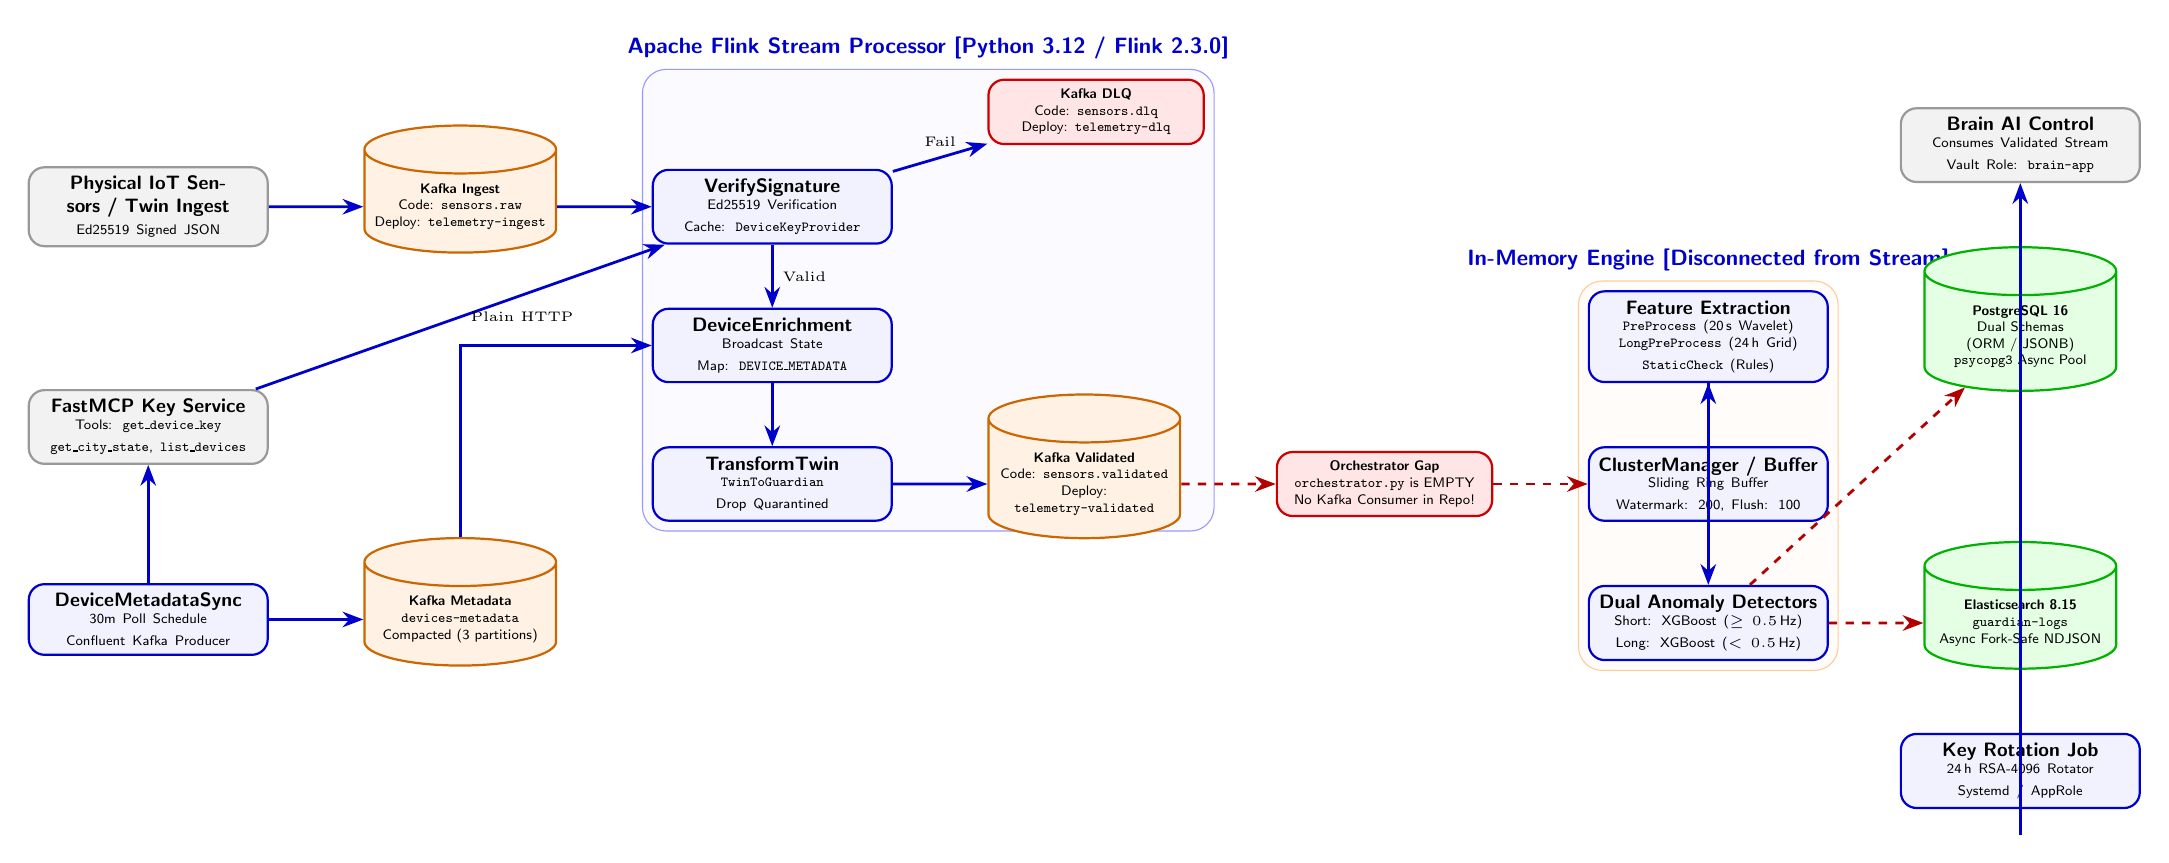
\begin{tikzpicture}[
    node distance=1.2cm and 1.5cm,
    box/.style={rectangle, draw=blue!80!black, fill=blue!5!white, rounded corners=2mm, text width=2.8cm, align=center, font=\sffamily\scriptsize, line width=0.8pt},
    extbox/.style={rectangle, draw=gray!80, fill=gray!10!white, rounded corners=2mm, text width=2.8cm, align=center, font=\sffamily\scriptsize, line width=0.8pt},
    queue/.style={cylinder, shape border rotate=90, draw=orange!80!black, fill=orange!10!white, aspect=0.25, text width=2.2cm, align=center, font=\sffamily\tiny, line width=0.8pt},
    db/.style={cylinder, shape border rotate=90, draw=green!70!black, fill=green!10!white, aspect=0.25, text width=2.2cm, align=center, font=\sffamily\tiny, line width=0.8pt},
    alert/.style={rectangle, draw=red!80!black, fill=red!10!white, rounded corners=2mm, text width=2.5cm, align=center, font=\sffamily\tiny, line width=0.8pt},
    line/.style={-{Stealth[scale=1.0]}, draw=blue!80!black, line width=1pt},
    broken/.style={-{Stealth[scale=1.0]}, draw=red!70!black, line width=1pt, dashed},
    grouplabel/.style={font=\sffamily\bfseries\footnotesize, color=blue!80!black}
]

% External Twin
\node[extbox] (twin_prod) {\textbf{Physical IoT Sensors / Twin Ingest}\\\tiny Ed25519 Signed JSON};
\node[extbox, below=1.8cm of twin_prod] (mcp_server) {\textbf{FastMCP Key Service}\\\tiny Tools: \texttt{get\_device\_key}\\\texttt{get\_city\_state}, \texttt{list\_devices}};

% Ingestion
\node[queue, right=1.2cm of twin_prod] (kafka_raw) {\textbf{Kafka Ingest}\\\tiny Code: \texttt{sensors.raw}\\\tiny Deploy: \texttt{telemetry-ingest}};
\node[box, right=1.2cm of kafka_raw] (flink_sig) {\textbf{VerifySignature}\\\tiny Ed25519 Verification\\\tiny Cache: \texttt{DeviceKeyProvider}};
\node[box, below=0.8cm of flink_sig] (flink_enrich) {\textbf{DeviceEnrichment}\\\tiny Broadcast State\\\tiny Map: \texttt{DEVICE\_METADATA}};
\node[box, below=0.8cm of flink_enrich] (flink_trans) {\textbf{TransformTwin}\\\tiny \texttt{TwinToGuardian}\\\tiny Drop Quarantined};

% DLQ & Validated
\node[alert, above right=0.3cm and 1.2cm of flink_sig] (kafka_dlq) {\textbf{Kafka DLQ}\\\tiny Code: \texttt{sensors.dlq}\\\tiny Deploy: \texttt{telemetry-dlq}};
\node[queue, right=1.2cm of flink_trans] (kafka_val) {\textbf{Kafka Validated}\\\tiny Code: \texttt{sensors.validated}\\\tiny Deploy: \texttt{telemetry-validated}};

% Metadata sync
\node[box, below=1.5cm of mcp_server] (meta_sync) {\textbf{DeviceMetadataSync}\\\tiny 30m Poll Schedule\\\tiny Confluent Kafka Producer};
\node[queue, right=1.2cm of meta_sync] (kafka_meta) {\textbf{Kafka Metadata}\\\tiny \texttt{devices-metadata}\\\tiny Compacted (3 partitions)};

% Disconnect Gap
\node[alert, right=1.2cm of kafka_val] (orchestrator_gap) {\textbf{Orchestrator Gap}\\\tiny \texttt{orchestrator.py} is EMPTY\\\tiny No Kafka Consumer in Repo!};

% Buffers & Feature Extraction
\node[box, right=1.2cm of orchestrator_gap] (mgr_buffers) {\textbf{ClusterManager / Buffer}\\\tiny Sliding Ring Buffer\\\tiny Watermark: 200, Flush: 100};
\node[box, above=0.8cm of mgr_buffers] (pipelines) {\textbf{Feature Extraction}\\\tiny \texttt{PreProcess} (20\,s Wavelet)\\\tiny \texttt{LongPreProcess} (24\,h Grid)\\\tiny \texttt{StaticCheck} (Rules)};
\node[box, below=0.8cm of mgr_buffers] (ai_inference) {\textbf{Dual Anomaly Detectors}\\\tiny Short: XGBoost ($\ge 0.5$\,Hz)\\\tiny Long: XGBoost ($< 0.5$\,Hz)};

% Persistence & Logs
\node[db, right=1.2cm of pipelines] (postgres_db) {\textbf{PostgreSQL 16}\\\tiny Dual Schemas (ORM / JSONB)\\\tiny \texttt{psycopg3} Async Pool};
\node[db, right=1.2cm of ai_inference] (elastic_db) {\textbf{Elasticsearch 8.15}\\\tiny \texttt{guardian-logs}\\\tiny Async Fork-Safe NDJSON};

% Brain & Vault
\node[extbox, above=0.8cm of postgres_db] (brain_layer) {\textbf{Brain AI Control}\\\tiny Consumes Validated Stream\\\tiny Vault Role: \texttt{brain-app}};
\node[box, below=0.8cm of elastic_db] (vault_rot) {\textbf{Key Rotation Job}\\\tiny 24\,h RSA-4096 Rotator\\\tiny Systemd / AppRole};

% Connections
\draw[line] (twin_prod) -- (kafka_raw);
\draw[line] (kafka_raw) -- (flink_sig);
\draw[line] (flink_sig) -- node[right]{\tiny Valid} (flink_enrich);
\draw[line] (flink_sig) -- node[above]{\tiny Fail} (kafka_dlq);
\draw[line] (flink_enrich) -- (flink_trans);
\draw[line] (flink_trans) -- (kafka_val);
\draw[line] (mcp_server) -- node[right]{\tiny Plain HTTP} (flink_sig);
\draw[line] (meta_sync) -- (mcp_server);
\draw[line] (meta_sync) -- (kafka_meta);
\draw[line] (kafka_meta) |- (flink_enrich);

% Broken Links
\draw[broken] (kafka_val) -- (orchestrator_gap);
\draw[broken] (orchestrator_gap) -- (mgr_buffers);
\draw[line] (mgr_buffers) -- (pipelines);
\draw[line] (pipelines) -- (ai_inference);
\draw[broken] (ai_inference) -- (postgres_db);
\draw[broken] (ai_inference) -- (elastic_db);
\draw[line] (vault_rot) -- ++(0,-0.8) -| (brain_layer);

% Grouping Boundaries
\begin{scope}[on background layer]
    \node[draw=blue!40, fill=blue!2!white, rounded corners=3mm, fit=(flink_sig) (flink_trans) (kafka_dlq), label={[grouplabel]above:Apache Flink Stream Processor [Python 3.12 / Flink 2.3.0]}] {};
    \node[draw=orange!40, fill=orange!2!white, rounded corners=3mm, fit=(mgr_buffers) (pipelines) (ai_inference), label={[grouplabel]above:In-Memory Engine [Disconnected from Stream]}] {};
\end{scope}

\end{tikzpicture}
}
\caption{Reconstructed System Architecture \& End-to-End Execution Flow (Evidence Grounded)}
\label{fig:real_arch_flow}
\end{figure}

\section{Layer-by-Layer Architectural Decomposition}

\subsection{Digital Twin Layer (External Ingestion Producer)}
\begin{itemize}[leftmargin=*]
  \item \textbf{Purpose:} Ingestion source representing the physical IoT instrumentation layer. Transmits signed serialized telemetry packets and exposes metadata/keys via FastMCP.
  \item \textbf{Interface Contracts:} Inbound telemetry via Kafka topic \texttt{telemetry-ingest} (code reference: \texttt{sensors.raw}). FastMCP Server listening at \texttt{http://host.docker.internal:8000/sse}.
  \item \textbf{Authentication \& Cryptography:} Payloads are digitally signed using Ed25519. The digital signature is transmitted in base64 string format in field \texttt{sig}.
  \item \textbf{Failure Mode:} If the Digital Twin sends corrupted JSON or an unparseable signature, \texttt{VerifySignature} routes the packet to DLQ with error code \texttt{E100\_DESERIALIZE} or \texttt{E200\_BAD\_SIGNATURE}.
\end{itemize}

\subsection{Guardian Layer (Internal Processing Core)}
The Guardian Layer is internally organized into six operational subsystems:
\begin{enumerate}
  \item \textbf{Stream Validation \& Enrichment Subsystem (\texttt{consumer\_producer/kafka\_consumer/}):}
  \begin{itemize}
    \item \texttt{VerifySignature}: Strips signature \texttt{sig}, canonicalizes JSON payload (\texttt{sort\_keys=True, separators=(',', ':')}), resolves public key via \texttt{DeviceKeyProvider}, and verifies with Ed25519.
    \item \texttt{DeviceEnrichment}: Implements Flink \texttt{KeyedBroadcastProcessFunction} joining sensor events keyed by \texttt{device\_id} against dynamic \texttt{devices-metadata} broadcast state.
    \item \texttt{EnrichAndTransform}: Parses enriched JSON into Pydantic domain models (\texttt{Sensor}), triggering automatic physical boundary and timestamp validation via \texttt{SensorValidator}.
    \item \texttt{TransformTwin}: Anti-Corruption Layer converting external \texttt{TwinSensorReading} models into unified internal \texttt{Sensor} entities. Drops quarantined/isolated nodes via \texttt{TransformDropped}.
  \end{itemize}
  \item \textbf{Metadata Synchronization Daemon (\texttt{consumer\_producer/kafka\_producer/}):}
  Periodic background synchronizer running every 30 minutes (\texttt{SYNC\_INTERVAL = 1800\,s}). Queries MCP tools \texttt{get\_city\_state} and \texttt{list\_devices}, detects topological differences, and produces compacted updates to \texttt{devices-metadata}.
  \item \textbf{Buffer Management Subsystem (\texttt{managers/}):}
  Hierarchical in-memory buffer topology. \texttt{ClusterManager} groups multiple \texttt{BufferManager} instances by \texttt{cluster\_id}. Each \texttt{Buffer} maintains a sliding window with a default high-watermark of 200 readings and an automatic atomic flush size of 100 readings dispatched into a thread-safe \texttt{FlushChannel}.
  \item \textbf{Signal Decomposition \& Feature Pipelines (\texttt{pipelines/}):}
  \begin{itemize}
    \item \texttt{StaticCheck}: Instantaneous physical boundary filters (\texttt{out\_of\_range}), silence detection (\texttt{sensor\_is\_down} after 10\,s), and gross spatial divergence (\texttt{spoofed\_data} against $k=5$ cluster neighbors).
    \item \texttt{PreProcess}: 20\,s short-window feature extraction running Robust $Z$-score scaling ($\text{MAD} \times 1.4826$), sign-flip oscillation rates, difference kurtosis, and Haar wavelet energy decoupling.
    \item \texttt{LongPreProcess}: 24\,h long-window batch processing resampling readings onto a 300\,s regular time-grid, calculating trend-to-scatter linear regression ratios, flat-run share, and neighbor slope deltas.
  \end{itemize}
  \item \textbf{Inference Detectors (\texttt{ai/inference/}):}
  \texttt{BaselineModel} executing multiclass CPU-optimized XGBoost decision trees. \texttt{AnomalyDetector} evaluates sensors sampling at $\ge 0.5$\,Hz against rate-adaptive threshold bands. \texttt{LongAnomalyDetector} evaluates slow telemetry ($< 0.5$\,Hz) across 24\,h windows.
  \item \textbf{Persistence \& Observability (\texttt{storage/}, \texttt{utils/}):}
  PostgreSQL 16 relational storage backed by \texttt{psycopg3} connection pooling (\texttt{AsyncConnectionPool}) and \texttt{AsyncElasticSearchHandler} providing non-blocking, fork-safe NDJSON bulk shipping to Elasticsearch.
\end{enumerate}

\subsection{Brain Layer (External Supervisory Control)}
\begin{itemize}[leftmargin=*]
  \item \textbf{Purpose:} Downstream supervisory command layer executing autonomous urban actuation (e.g., sluice gate deployment, flood barrier activation).
  \item \textbf{Interface Contracts:} Consumes validated sensor telemetry from Kafka topic \texttt{telemetry-validated} and anomaly feeds from \texttt{spatial-anomalies} via Kafka SASL principal \texttt{User:executioner} and \texttt{User:brain}.
  \item \textbf{Security Policies:} Bound to Vault policy \texttt{brain-app.hcl}, granting read-only access to \texttt{secret/data/comm/brain/*}.
\end{itemize}

\section{Inter-Layer Contracts \& Interface Mappings}

\subsection{Kafka Topic Architecture \& Mappings}
A critical technical divergence exists between topic names declared in deployment scripts, documentation, and PyFlink code (Table~\ref{tab:kafka_topic_contracts}).

\begin{table}[htbp]
\centering
\small
\caption{Kafka Topic Naming, Partitioning, Replication, and Access Contracts}
\label{tab:kafka_topic_contracts}
\begin{tabularx}{\textwidth}{lXcccX}
\toprule
\textbf{Documented Topic} & \textbf{Deployed Topic Name} & \textbf{Code Topic Name} & \textbf{Part.} & \textbf{Repl.} & \textbf{Configured Retention / ACLs} \\
\midrule
\texttt{sensors.raw} & \texttt{telemetry-ingest} & \texttt{sensors.raw} & 6 & 3 & 7 days; \texttt{twin} (W), \texttt{guardian} (R) \\
\texttt{sensors.validated} & \texttt{telemetry-validated} & \texttt{sensors.validated} & 6 & 3 & 7 days; \texttt{guardian} (W), \texttt{executioner} (R) \\
\texttt{sensors.dlq} & \texttt{telemetry-dlq} & \texttt{sensors.dlq} & 3 & 3 & 30 days; \texttt{guardian} (W), \texttt{executioner} (R) \\
\texttt{devices-metadata} & \texttt{devices-metadata} & \texttt{devices-metadata} & 3 & 3 & Compacted; \texttt{broadcast} (W), \texttt{guardian} (R) \\
\textit{Undocumented} & \texttt{video-frames-ingest} & \textit{None} & 4 & 3 & 1 hour, max 5\,MB; \texttt{twin} (W), \texttt{guardian} (R) \\
\textit{Undocumented} & \texttt{spatial-anomalies} & \textit{None} & 3 & 3 & 7 days; \texttt{guardian} (W), \texttt{executioner} (R) \\
\bottomrule
\end{tabularx}
\end{table}

\subsection{Structured Error Codes}
Every stream validation failure emits a standardized JSON document to the Dead-Letter Queue (DLQ) generated by \texttt{reject(code, detail, raw)} in \texttt{jobs/functions.py}:
\begin{table}[htbp]
\centering
\small
\caption{Guardian Dead-Letter Queue (DLQ) Error Code Catalog}
\label{tab:error_codes}
\begin{tabularx}{\textwidth}{llXl}
\toprule
\textbf{Error Code} & \textbf{Emitting Component} & \textbf{Trigger Condition} & \textbf{Destination} \\
\midrule
\texttt{E100\_DESERIALIZE} & \texttt{VerifySignature} & Raw payload is not valid JSON or not a JSON object & \texttt{sensors.dlq} \\
\texttt{E200\_BAD\_SIGNATURE} & \texttt{VerifySignature} & Cryptographic Ed25519 signature mismatch & \texttt{sensors.dlq} \\
\texttt{E201\_UNKNOWN\_DEVICE} & \texttt{VerifySignature} & Device public key not returned by FastMCP server & \texttt{sensors.dlq} \\
\texttt{E300\_SCHEMA} & \texttt{EnrichAndTransform} & Pydantic validation failure against \texttt{Sensor} schema & \texttt{sensors.dlq} \\
\texttt{E320\_UNKNOWN\_STATUS} & \texttt{TransformTwin} & Payload status string not in \texttt{TwinStatus} enum & \textbf{Lost} (F-07) \\
\texttt{E400\_SENSOR\_VALIDATION} & \texttt{EnrichAndTransform} & Physical boundary or timestamp validation failure & \texttt{sensors.dlq} \\
\texttt{E500\_ENRICHMENT} & \texttt{EnrichAndTransform} & Internal enrichment backend exception & \texttt{sensors.dlq} \\
\bottomrule
\end{tabularx}
\end{table}

\subsection{FastMCP Edge Tool Specifications}
The Guardian Layer client connects to FastMCP via \texttt{McpToolClient} (\texttt{mcp\_client/client.py}):
\begin{itemize}[leftmargin=*]
  \item \texttt{get\_device\_key(device\_id: str) -> str}: Retrieves base64-encoded Ed25519 public key (32 raw bytes or SPKI DER structure). Wrapped in \texttt{DeviceKeyProvider} with a 300\,s positive TTL and a 30\,s negative TTL.
  \item \texttt{get\_city\_state() -> dict}: Returns geographical urban zoning map (\texttt{"zones": \{...\}}).
  \item \texttt{list\_devices(zone\_id: str) -> list[dict]}: Returns device metadata containing coordinates (\texttt{lat}, \texttt{lon}), measurement bounds (\texttt{min\_val}, \texttt{max\_val}), and physical units (\texttt{unit}).
\end{itemize}

\subsection{HashiCorp Vault Secret Paths}
Inter-service cryptographic material is partitioned into unidirectional KV v2 endpoints:
\begin{itemize}[leftmargin=*]
  \item \texttt{secret/data/comm/<OWNER>/<PEER>/private}: Readable strictly by \texttt{<OWNER>-app}. Contains RSA-4096 private key PEM, key ID (\texttt{kid}), and timestamp \texttt{active\_after}.
  \item \texttt{secret/data/comm/<OWNER>/<PEER>/public}: Readable strictly by \texttt{<PEER>-app}. Contains RSA-4096 public key PEM, key ID (\texttt{kid}), creation timestamp, and SHA-256 fingerprint.
\end{itemize}

\section{Data Lifecycle and Persistence Architecture}
\begin{itemize}[leftmargin=*]
  \item \textbf{Raw Telemetry:} Persisted in Kafka broker commit logs (\texttt{/var/lib/kafka/data}) with a 7-day retention period (\texttt{retention.ms=604800000}) and replication factor of 3.
  \item \textbf{Sliding Window State:} Resides exclusively in volatile process memory (\texttt{Buffer.readings: list[Sensor]}). Watermark limits allow up to 200 items in RAM. \textbf{Unflushed data is destroyed on process crash or container eviction.}
  \item \textbf{Relational Database Persistence:} Two divergent persistence models exist in the codebase:
  \begin{itemize}
    \item \textit{Relational ORM Model (\texttt{storage/models.py}):} 4 typed tables: \texttt{raw\_readings}, \texttt{processed\_readings}, \texttt{transformed\_windows}, \texttt{model\_outputs}. Supports multi-row batch inserts via \texttt{insert\_batch}.
    \item \textit{JSONB Model (\texttt{storage/connections/postgress.py}):} 3 JSONB tables: \texttt{sensors}, \texttt{sensor\_summaries}, \texttt{verdicts}.
  \end{itemize}
  Neither model implements database partitioning, data retention TTLs, or automated archival.
  \item \textbf{Log Persistence:} Bulk JSON log documents dispatched to Elasticsearch index \texttt{guardian-logs} with no defined Index Lifecycle Management (ILM) policy.
\end{itemize}

\section{Deployment, Operations \& Observability}
The system is orchestrated via \texttt{docker-compose.yml} declaring 10 services (Table~\ref{tab:compose_inventory}).

\begin{table}[htbp]
\centering
\small
\caption{Docker Compose Service Inventory \& Operational Healthchecks}
\label{tab:compose_inventory}
\begin{tabularx}{\textwidth}{llXl}
\toprule
\textbf{Service Name} & \textbf{Base Image} & \textbf{Network / Port Bindings} & \textbf{Healthcheck Mechanism} \\
\midrule
\texttt{kafka-1, 2, 3} & \texttt{apache/kafka:4.3.1} & Host \texttt{29094-29096}, Inter-broker \texttt{19094} & Broker API quorum check \\
\texttt{kafka-init} & \texttt{apache/kafka:4.3.1} & Transient init container (exits on complete) & None (Runs \texttt{kafka-init.sh}) \\
\texttt{postgres} & \texttt{postgres:16-alpine} & Host \texttt{127.0.0.1:5432:5432} & \texttt{pg\_isready -U guardian} \\
\texttt{elasticsearch} & \texttt{elasticsearch:8.15.0} & Host \texttt{127.0.0.1:9200:9200} & \texttt{curl -u elastic:\$PASSWORD} \\
\texttt{jobmanager} & \texttt{sensor-flink:1.20} & Host \texttt{127.0.0.1:8081:8081} & \texttt{curl http://localhost:8081/overview} \\
\texttt{taskmanager} & \texttt{sensor-flink:1.20} & Internal cluster only (2 replicas, 6 slots) & Managed by JobManager RPC \\
\texttt{job-submitter} & \texttt{sensor-flink:1.20} & Transient Flink job launcher & None \\
\texttt{device-producer} & Built via \texttt{Dockerfile.producer} & Internal \texttt{shared-backend} & None \\
\bottomrule
\end{tabularx}
\end{table}

\section{Component Mapping Table}
Table~\ref{tab:mapping_verification} compares components documented in \texttt{TECHNICAL\_DOCUMENTATION.md} against verified source files.

\begin{table}[htbp]
\centering
\small
\caption{Documented Architecture vs.\ Source Code Implementation Mapping}
\label{tab:mapping_verification}
\begin{tabularx}{\textwidth}{lXll}
\toprule
\textbf{Documented Component} & \textbf{Actual Source Path} & \textbf{Code Status} & \textbf{Discrepancy Note} \\
\midrule
Signature Verification & \texttt{src/guardian\_layer/consumer\_producer/.../signature.py} & \textbf{Matches} & Ed25519 signature checks match code \\
MCP Key Resolution & \texttt{src/guardian\_layer/mcp\_client/client.py} & \textbf{Matches} & Uses FastMCP SSE Client \\
Metadata Broadcast & \texttt{src/guardian\_layer/consumer\_producer/.../functions.py} & \textbf{Matches} & Flink KeyedBroadcastProcessFunction \\
Twin-to-Guardian Trans. & \texttt{src/guardian\_layer/data\_transformer/transformer/twin\_v1.py} & \textbf{Matches} & Class decorator registration \\
Sliding Ring Buffers & \texttt{src/guardian\_layer/managers/buffer\_manger.py} & \textbf{Matches} & Threading lock protected \\
Short-Window Anomaly & \texttt{src/guardian\_layer/ai/inference/detector.py} & \textbf{Matches} & XGBoost multiclass model \\
Long-Window Anomaly & \texttt{src/guardian\_layer/ai/inference/long\_detector.py} & \textbf{Matches} & 24\,h resampled grid inference \\
PostgreSQL Persistence & \texttt{src/guardian\_layer/storage/database.py} & \textbf{Matches} & SQLAlchemy batch insertion \\
Async Logging Handler & \texttt{src/guardian\_layer/utils/elastic.py} & \textbf{Matches} & Fork-safe bounded queue bulk log \\
Vault Key Rotator & \texttt{vault/rotate\_keys.py} & \textbf{Matches} & 24\,h RSA rotation with 1\,h overlap \\
\textbf{Pipeline Orchestrator} & \texttt{src/guardian\_layer/orchestrator.py} & \textbf{Differs} & \textbf{File exists but is 0 bytes (Empty)} \\
\textbf{Flink Dockerfile} & \texttt{Dockerfile.flink} & \textbf{Missing} & \textbf{Referenced in Compose but absent} \\
\textbf{Vault Compose Svc} & \texttt{docker-compose.yml} & \textbf{Missing} & \textbf{Documented Raft cluster absent} \\
\textbf{Stream Wire Topics} & \texttt{job.py} vs.\ \texttt{kafka-init.sh} & \textbf{Differs} & \textbf{Topic names do not align} \\
\bottomrule
\end{tabularx}
\end{table}

\section{Documentation Gaps and Inconsistencies}
\begin{enumerate}[leftmargin=*]
  \item \textbf{D-01 (Maturity Misrepresentation):} Documentation states the system is a ``Production-Ready Core Layer'' (line 5), whereas \texttt{orchestrator.py} is empty, stream topics diverge, and the Flink job crashes on schema evaluation.
  \item \textbf{D-02 (Topic Name Divergence):} Documentation diagrams cite \texttt{sensors.raw}, \texttt{sensors.validated}, and \texttt{sensors.dlq}; \texttt{kafka-init.sh} provisions \texttt{telemetry-ingest}, \texttt{telemetry-validated}, and \texttt{telemetry-dlq}.
  \item \textbf{D-03 (Version Inconsistency):} Stack table claims Apache Flink 2.3.0 and PyFlink 1.20; \texttt{uv.lock} pins \texttt{apache-flink==2.3.0}, \texttt{docker-compose.yml} specifies image tag \texttt{1.20}, and the SQL connector jar is 2.3.0.
  \item \textbf{D-04 (Absolute Claims Contradicted):} Terms such as ``unbreachable defensive boundary'', ``exactly-once'', and ``zero data loss'' are contradicted by volatile in-memory ring buffers and plaintext network transport.
  \item \textbf{D-05 (Dependency Version Drift):} Ruff is documented as 0.16.9 (lock: 0.17.3); Mypy as 2.3.1 (lock: 2.4.1); SQLAlchemy as 2.0 (lock: 2.1.6); Psycopg as 3.2 (lock: 3.3.6).
  \item \textbf{D-06 (Concurrency Documentation Error):} Documentation asserts that \texttt{Buffer.\_lock} is a ``re-entrant \texttt{threading.Lock}''; standard Python \texttt{threading.Lock} is non-reentrant.
  \item \textbf{D-07 (Unbounded Buffer Growth on Restore):} Documentation claims buffers are strictly bounded; \texttt{Buffer.restore()} prepends flushed batches directly into \texttt{self.readings} without enforcing the high-watermark.
  \item \textbf{D-08 (Vault Test Execution Reality):} Documentation claims tests execute against ``live or mock Vault APIs''; all 15 tests are unconditionally skipped unless an external live Vault cluster is manually provisioned.
  \item \textbf{D-09 (Alert Environment Key Discrepancy):} Security guides document \texttt{ALERT\_WEBHOOK\_URL}; \texttt{rotate\_keys.py} parses \texttt{GUARDIAN\_ROTATION\_URL}, \texttt{TWIN\_ROTATION\_URL}, and \texttt{BRAIN\_ROTATION\_URL}.
  \item \textbf{D-10 (Selective ML Reporting):} Documentation quotes 0.008 false alarms/sensor-day and 0.951 PR-AUC without disclosing that on real battery/flag anomalies, the model flags only 2.5\%--3.5\% of faults.
  \item \textbf{D-11 (Configuration Typo):} Compose file defines \texttt{Sync\_confgig} instead of \texttt{SYNC\_CONFIG}.
  \item \textbf{D-12 (Dual Storage Omission):} Documentation describes a 4-table SQLAlchemy schema but omits mention of the alternative JSONB schema class in \texttt{storage/connections/postgress.py}.
\end{enumerate}

% ==============================================================================
% CHAPTER 4: PART B - SECURITY MEASURES
% ==============================================================================
\chapter{PART B: Security Measures}

\section{Threat Modeling \& Trust Boundaries (STRIDE Analysis)}
The Guardian Layer operates across six discrete trust boundaries. Table~\ref{tab:stride_matrix} details the STRIDE threat matrix derived from concrete code inspection.

\begin{center}
\small
\begin{longtable}{p{2.2cm}p{4cm}p{2.5cm}p{3.5cm}p{3.5cm}}
\caption{STRIDE Threat Modeling Across Guardian Layer Interfaces} \label{tab:stride_matrix} \\
\toprule
\textbf{STRIDE Category} & \textbf{Threat Description} & \textbf{Affected Interface} & \textbf{Mitigation in Code} & \textbf{Residual Risk / Gap} \\
\midrule
\endfirsthead
\multicolumn{5}{c}{\small\textsf{\tablename\ \thetable\ -- Continued from previous page}} \\
\toprule
\textbf{STRIDE Category} & \textbf{Threat Description} & \textbf{Affected Interface} & \textbf{Mitigation in Code} & \textbf{Residual Risk / Gap} \\
\midrule
\endhead
\bottomrule
\multicolumn{5}{r}{\small\textsf{Continued on next page...}} \\
\endfoot
\bottomrule
\endlastfoot
\textbf{Spoofing} & Adversary injects fabricated telemetry masquerading as a field sensor. & Device $\rightarrow$ Kafka \texttt{sensors.raw} & Ed25519 digital signature verified in \texttt{VerifySignature}. & Low if private keys are protected; FastMCP key service can be spoofed. \\
\midrule
\textbf{Tampering} & Payload modified in flight between IoT edge and ingestion broker. & Device $\rightarrow$ Kafka & Signature covers canonical JSON payload bytes. & Mitigated by Ed25519; however, transport is cleartext (eavesdropping risk). \\
\midrule
\textbf{Repudiation} & Rogue sensor denies transmitting erroneous or hazardous data. & Device $\rightarrow$ Kafka & Non-repudiation guaranteed by asymmetric Ed25519 keys. & Mitigated if device private key is hardware-bound (TPM/HSM). \\
\midrule
\textbf{Information Disclosure} & Plaintext sensor readings and credentials intercepted on wire. & All Kafka, MCP \& Elasticsearch links & None. Network transport uses \texttt{SASL\_PLAINTEXT} and HTTP. & \textbf{CRITICAL.} Complete exposure of credentials and telemetry to network sniffers. \\
\midrule
\textbf{Denial of Service} & High-rate telemetry flood exhausts broker or Flink worker memory. & Kafka $\rightarrow$ Flink $\rightarrow$ In-Memory Buffer & Sliding ring buffer drops oldest readings when full; backpressure channel. & Buffer overflow during downstream outages triggers CPU spin in \texttt{BufferManager}. \\
\midrule
\textbf{Elevation of Privilege} & Compromised microservice accesses lateral communication keys. & Services $\rightarrow$ HashiCorp Vault & Least-privilege HCL policies restrict token access to own paths. & Mitigated by Vault AppRole; however, rotator script writes keys non-atomically. \\
\bottomrule
\end{longtable}
\end{center}

\section{Security Control Inventory}
Table~\ref{tab:control_inventory} maps all technical controls implemented in the repository against NIST SP 800-207 (Zero Trust Architecture), NIST SP 800-57 (Key Management), ISO/IEC 27001:2022 Annex A, and OWASP ASVS 4.0.3.

\begin{center}
\scriptsize
\begin{longtable}{llp{4.2cm}llc}
\caption{Comprehensive Security Control Inventory \& Standard Mapping} \label{tab:control_inventory} \\
\toprule
\textbf{Control Domain} & \textbf{Layer} & \textbf{Technical Mechanism} & \textbf{Source File Reference} & \textbf{Standard Mapping} & \textbf{Status} \\
\midrule
\endfirsthead
\multicolumn{6}{c}{\small\textsf{\tablename\ \thetable\ -- Continued from previous page}} \\
\toprule
\textbf{Control Domain} & \textbf{Layer} & \textbf{Technical Mechanism} & \textbf{Source File Reference} & \textbf{Standard Mapping} & \textbf{Status} \\
\midrule
\endhead
\bottomrule
\multicolumn{6}{r}{\small\textsf{Continued on next page...}} \\
\endfoot
\bottomrule
\endlastfoot
\textbf{Device Auth.} & Ingest & Ed25519 signature verification on canonical JSON & \texttt{jobs/signature.py} & NIST 800-207 §3.1 & \textbf{Implemented} \\
\textbf{Key Management} & Edge & FastMCP key distribution with positive/negative TTL & \texttt{mcp\_client/client.py} & NIST 800-57 Part 1 & \textbf{Partial} \\
\textbf{Key Rotation} & Inter-Svc & 24\,h RSA-4096 key rotation with 1\,h overlap window & \texttt{vault/rotate\_keys.py} & NIST 800-57 §5.3.6 & \textbf{Implemented} \\
\textbf{Secret Isolation} & Infra & AppRole tokens (15\,m TTL, 1\,h max renew, 24\,h secret\_id) & \texttt{vault/setup\_policies.py} & ISO 27001 A.9.4.2 & \textbf{Implemented} \\
\textbf{Least Privilege} & Storage & Path-scoped Vault policies (read-only per peer) & \texttt{vault/policies/*.hcl} & NIST 800-207 §2.1 & \textbf{Implemented} \\
\textbf{Broker Security} & Message & SASL PLAIN authentication with StandardAuthorizer & \texttt{docker-compose.yml} & OWASP ASVS V2.1 & \textbf{Partial} \\
\textbf{Transport Security} & Network & Enforced TLS / HTTPS encryption & None & ISO 27001 A.13.1 & \textbf{Absent} \\
\textbf{Input Validation} & Pipeline & Strict Pydantic models with physical boundary validation & \texttt{utils/sensor\_verification.py} & OWASP ASVS V5.1 & \textbf{Implemented} \\
\textbf{Dead-Letter Queue} & Stream & Structured error tagging and side-output routing & \texttt{jobs/functions.py} & OWASP ASVS V11.1 & \textbf{Implemented} \\
\textbf{Anti-Replay} & Edge & Nonce, timestamp freshness, and packet order checks & \texttt{pipelines/preprocess.py} & OWASP ASVS V3.6 & \textbf{Partial} \\
\textbf{Audit Logging} & Logging & Async NDJSON bulk delivery to Elasticsearch & \texttt{utils/elastic.py} & ISO 27001 A.12.4 & \textbf{Implemented} \\
\textbf{Buffer Protection} & Concurrency & Atomic restore of unpersisted batches on backpressure & \texttt{managers/buffer\_manger.py} & OWASP ASVS V11.2 & \textbf{Implemented} \\
\textbf{ML Integrity} & AI Core & Safe JSON model serialization (pickle prohibited) & \texttt{ai/inference/model.py} & OWASP ML Top 10 & \textbf{Implemented} \\
\textbf{Supply Chain} & Build & Deterministic SHA-256 package locking via \texttt{uv.lock} & \texttt{uv.lock} & ISO 27001 A.14.2 & \textbf{Implemented} \\
\end{longtable}
\end{center}

\subsection{Detailed Analysis Across Security Domains}

\subsubsection{1. Device Authentication \& Payload Signing}
Sensors sign the JSON representation of readings with Ed25519. \texttt{Ed25519SignatureVerifier} strips the \texttt{sig} attribute and sorts dictionary keys to create a canonical byte stream. Verification uses \texttt{cryptography.hazmat.primitives.asymmetric.ed25519}. If the first verification fails, the verifier executes a second pass with \texttt{refresh=True} to handle keys rotated at the edge.
\textbf{Vulnerability:} The verification does not assert a cryptographic timestamp or nonce inside the signed body. A captured valid packet can be replayed repeatedly across network boundaries without detection by \texttt{VerifySignature}.

\subsubsection{2. Key Management, Rotation \& Inter-Service Isolation}
Inter-service communication is secured by 4096-bit RSA keys managed via HashiCorp Vault KV v2:
\begin{itemize}[leftmargin=*]
  \item Daily rotation is automated via \texttt{vault/systemd/key-rotation.service} triggering \texttt{rotate\_keys.py} at 02:00 daily.
  \item \textbf{Overlap Logic:} When a new RSA keypair is generated, the public key is stored immediately in Vault with the new version number and unique key ID (\texttt{kid}). The private key is written with metadata attribute \texttt{active\_after = now + 3600\,s}.
  \item Senders inspect \texttt{active\_after} via \texttt{vault\_keys.signing\_key}. If the current time has not reached \texttt{active\_after}, the sender continues signing with version $N-1$.
  \item Receivers utilize \texttt{vault\_keys.verification\_keys}, which concurrently loads and trusts both version $N$ and version $N-1$.
  \item \textbf{Integrity Pinning:} Public keys stored in Vault include an explicit SHA-256 hex digest (\texttt{fingerprint}). \texttt{vault\_keys.\_checked()} computes \texttt{hashlib.sha256(data["public\_key"].encode()).hexdigest()} and raises \texttt{ValueError} if a byte diverges.
\end{itemize}

\subsubsection{3. Broker \& Network Security}
The broker infrastructure uses Apache Kafka 4.3.1 KRaft mode without ZooKeeper. \texttt{StandardAuthorizer} enforces default-deny ACLs (\texttt{KAFKA\_ALLOW\_EVERYONE\_IF\_NO\_ACL\_FOUND: "false"}).
\textbf{Vulnerability:} The security protocol is explicitly configured as \texttt{SASL\_PLAINTEXT}. User credentials (\texttt{user\_broker}, \texttt{user\_admin}, \texttt{user\_guardian}, \texttt{user\_twin}, \texttt{user\_brain}, \texttt{user\_broadcast}, \texttt{user\_executioner}) and all message payloads are transmitted in cleartext over TCP port 19094.

\subsubsection{4. Input Validation \& Edge Filtering}
Every instantiated \texttt{Sensor} executes \texttt{SensorValidator} during Pydantic post-initialization (\texttt{model\_post\_init}):
\begin{itemize}[leftmargin=*]
  \item Values must be finite floats (NaN and $\pm\infty$ rejected).
  \item Timestamps cannot be in the future relative to the processing node.
  \item Coordinates must be finite and within $[-90, 90]$ latitude and $[-180, 180]$ longitude. Lat and Lon must be provided together.
  \item Lower and upper range limits are validated (\texttt{upper\_range > lower\_range}).
\end{itemize}

\subsubsection{5. Machine Learning Security (Evasion, Poisoning \& Deserialization)}
\begin{itemize}[leftmargin=*]
  \item \textbf{Deserialization Safety:} \texttt{BaselineModel.save} and \texttt{load} utilize XGBoost's native JSON format (\texttt{model.json}), explicitly eradicating Python \texttt{pickle} vulnerabilities.
  \item \textbf{Adversarial Evasion:} The short-window model relies heavily on Robust $Z$-scores and sign-flip oscillations. However, research experiments (\texttt{research/short\_window/results.md}) establish that subtle injected noise (7\% recall on 1\,s data) and cluster-correlated spatial drift evade detection.
\end{itemize}

\section{Security Test Evidence \& Skipped Tests Analysis}
The repository includes automated security verification tests under \texttt{tests/vault\_keys/}:
\begin{itemize}[leftmargin=*]
  \item \texttt{test\_service\_reads\_only\_its\_own\_secrets}: Asserts that \texttt{guardian-app} receives \texttt{Forbidden} (HTTP 403) when attempting to access \texttt{twin} or \texttt{brain} private keys.
  \item \texttt{test\_services\_cannot\_write}: Confirms microservice AppRoles are restricted from writing secrets.
  \item \texttt{test\_rotator\_cannot\_read\_private\_keys}: Confirms the rotator role has \texttt{create, update} on secrets but cannot read private key values.
  \item \texttt{test\_signing\_key\_waits\_for\_overlap}: Validates that senders respect the 1-hour overlap window and peers accept both $N$ and $N-1$ keys.
  \item \texttt{test\_tampered\_public\_key\_is\_rejected}: Confirms that single-byte tampering of a public key triggers fingerprint validation exceptions.
\end{itemize}

\begin{callout}{Critical Test Harness Gap: 15 Skipped Security Tests}{red}
In standard CI execution and local development runs, \textbf{all 15 Vault security tests are unconditionally skipped}.
Fixture \texttt{admin} in \texttt{tests/vault\_keys/conftest.py} executes:
\begin{lstlisting}[language=Python]
addr, token = os.getenv("VAULT_TEST_ADDR"), os.getenv("VAULT_TEST_TOKEN")
if not (addr and token):
    pytest.skip("set VAULT_TEST_ADDR and VAULT_TEST_TOKEN")
\end{lstlisting}
Neither \texttt{docker-compose.yml} nor \texttt{.github/workflows/ci.yml} provisions a Vault test instance. Consequently, \textbf{none of the cryptographic isolation guarantees are verified during pull request CI builds}.
\end{callout}

\section{Residual Risks \& Evaluation of Documentation Claims}
\begin{itemize}[leftmargin=*]
  \item \textbf{Claim: ``Unbreachable defensive boundary'' $\rightarrow$ Refuted.} Cleartext network communications (Kafka, MCP, Elasticsearch) allow passive eavesdropping and man-in-the-middle key substitution.
  \item \textbf{Claim: ``Exactly-once state semantics'' $\rightarrow$ Refuted.} Flink Kafka sinks are explicitly instantiated with \texttt{DeliveryGuarantee.AT\_LEAST\_ONCE} (\texttt{kafka\_consumer/job.py} line 38).
  \item \textbf{Claim: ``Zero data loss / Zero-drop guarantee'' $\rightarrow$ Refuted.} While \texttt{Buffer.restore()} re-inserts unpersisted batches if the downstream queue is full, the entire buffer resides in volatile RAM. A container crash, out-of-memory kill, or host power failure results in irrevocable data loss.
\end{itemize}

% ==============================================================================
% CHAPTER 5: PART C - ARGUMENTATION OF TECHNICAL CHOICES
% ==============================================================================
\chapter{PART C: Argumentation of Technical Choices}

This section provides formal Architecture Decision Records (ADRs) evaluating the primary architectural, algorithmic, and engineering choices embodied in the Guardian Layer codebase.

\section{ADR-01: Apache Kafka with KRaft Consensus}
\begin{adrbox}{1}{Apache Kafka 4.3.1 with 3-Node KRaft Consensus}{Partially Justified}
\textbf{Context:} The system requires an event broker capable of ingesting high-throughput urban IoT telemetry, providing partitioned distribution, multi-tenant isolation, and persistent replayable logs.\\
\textbf{Alternatives Considered:} Apache Kafka with ZooKeeper; RabbitMQ (AMQP); Apache Pulsar; NATS JetStream.\\
\textbf{Justification:} KRaft eliminates the operational overhead, JVM memory consumption, and synchronization hazards of a separate ZooKeeper ensemble. The 3-node voter topology (\texttt{KAFKA\_CONTROLLER\_QUORUM\_VOTERS: "1@kafka-1:9093,2@kafka-2:9093,3@kafka-3:9093"}) guarantees continuous Raft consensus under the failure of any single node.\\
\textbf{Trade-offs \& Risks:} KRaft in Kafka 4.x is mature, but the current deployment enables \texttt{SASL\_PLAINTEXT} without TLS, exposing internal Raft control plane and client traffic to sniffing.\\
\textbf{Supporting Evidence:} \texttt{docker-compose.yml} lines 6--30; \texttt{tests/infra/test\_compose.py} lines 150--189.\\
\textbf{Reversibility:} Moderate. Topic and partition semantics are standard; migration to Pulsar or NATS requires rewriting broker connection libraries.\\
\textbf{Auditor Verdict:} \textbf{Partially Justified.} Operationally sound architecture undermined by the omission of TLS encryption.
\end{adrbox}

\section{ADR-02: Apache Flink (PyFlink) for Stream Processing}
\begin{adrbox}{2}{Apache Flink 2.3.0 / PyFlink Stream Verification}{Partially Justified}
\textbf{Context:} High-throughput stream ingestion requires stateful joins between fast-moving sensor readings and slow-moving metadata updates, with guaranteed low-latency signature checking.\\
\textbf{Alternatives Considered:} Kafka Streams (Java native); Faust (Python stream processor); Spark Structured Streaming; Native Asyncio Consumer.\\
\textbf{Justification:} Flink provides true event-driven streaming (unlike Spark micro-batching) and built-in Keyed Broadcast State (\texttt{KeyedBroadcastProcessFunction}), enabling dynamic broadcast of device metadata updates without querying an external cache on every event.\\
\textbf{Trade-offs \& Risks:} PyFlink introduces inter-process communication overhead between the Java JVM TaskManager and the Python runtime. The current deployment suffers from topic naming divergence and missing SASL client credentials.\\
\textbf{Supporting Evidence:} \texttt{src/guardian\_layer/consumer\_producer/kafka\_consumer/job.py}; \texttt{docker-compose.yml} lines 42--75.\\
\textbf{Reversibility:} Low. Deeply integrated into Flink execution APIs and broadcast state descriptors.\\
\textbf{Auditor Verdict:} \textbf{Partially Justified.} Architecturally appropriate for stateful streaming, but runtime implementation is currently broken and untested.
\end{adrbox}

\section{ADR-03: HashiCorp Vault with AppRole \& Automated 24\,h Rotation}
\begin{adrbox}{3}{HashiCorp Vault with AppRole \& Daily Key Rotation}{Justified}
\textbf{Context:} Zero-trust principles dictate that inter-service communication keys (Guardian, Twin, Brain) must be isolated, short-lived, and automatically rotated without downtime.\\
\textbf{Alternatives Considered:} Static credentials in environment variables; Kubernetes Secrets; AWS Secrets Manager / KMS; SOPS encrypted repository files.\\
\textbf{Justification:} AppRole authentication provides automated token issuance with bounded lifetimes (15\,m TTL, 1\,h maximum renewal). Path-scoped HCL policies enforce absolute default-deny boundaries. The 1-hour overlap window ensures continuous decryption capability across rotation boundaries.\\
\textbf{Trade-offs \& Risks:} Adds operational complexity (Vault unseal process, AppRole secret ID distribution). Rotator script executes key updates sequentially rather than in an atomic Vault transaction.\\
\textbf{Supporting Evidence:} \texttt{vault/rotate\_keys.py}; \texttt{vault/policies/*.hcl}; \texttt{tests/vault\_keys/test\_vault\_policies.py}.\\
\textbf{Reversibility:} High. Cryptographic keys can be loaded from alternative key-management endpoints with minimal interface changes.\\
\textbf{Auditor Verdict:} \textbf{Justified.} Exemplary implementation of zero-trust secret management and automated key lifecycle engineering.
\end{adrbox}

\section{ADR-04: Dual Cryptographic Architecture (Ed25519 vs.\ RSA-4096)}
\begin{adrbox}{4}{Ed25519 for Edge Signatures vs.\ RSA-4096 for Inter-Service Traffic}{Justified}
\textbf{Context:} Edge IoT sensors have constrained CPU, memory, and bandwidth, requiring compact signatures with ultra-fast verification. Server-to-server microservices require high-entropy asymmetric isolation.\\
\textbf{Alternatives Considered:} Universal RSA-2048/4096; Universal ECDSA (NIST P-256); HMAC-SHA256 symmetric pre-shared keys.\\
\textbf{Justification:} Ed25519 signatures are 64 bytes with 32-byte public keys, verifying in microseconds on resource-constrained microcontrollers. RSA-4096 with OAEP padding and SHA-256 provides military-grade confidentiality and asymmetric signing for inter-service communication across datacenters.\\
\textbf{Trade-offs \& Risks:} Two distinct cryptographic code paths must be maintained. Device keys cannot be rotated via Vault and must be fetched via FastMCP.\\
\textbf{Supporting Evidence:} \texttt{signature.py} lines 6--9; \texttt{vault\_keys.py} lines 19--50; \texttt{helpers.py} lines 30--54.\\
\textbf{Reversibility:} High. Verification interfaces encapsulate the cryptographic primitives behind unified abstractions.\\
\textbf{Auditor Verdict:} \textbf{Justified.} Clean, well-reasoned cryptographic separation balancing edge efficiency against backend security.
\end{adrbox}

\section{ADR-05: In-Memory Ring Buffering with Atomic Rollback}
\begin{adrbox}{5}{In-Memory Ring Buffers with Atomic Flush Rollback}{Partially Justified}
\textbf{Context:} Downstream ML feature extraction requires aggregated windows of 100--200 sensor readings. Single-event insertions into databases or queues create severe I/O bottlenecks.\\
\textbf{Alternatives Considered:} Redis sliding window sorted sets; RocksDB embedded key-value store; SQLite WAL memory tables; Direct Kafka consumer windowing.\\
\textbf{Justification:} Pure in-memory Python dataclass buffers (\texttt{Buffer}) execute additions in 2.75\,$\mu$s and batch flushes in 15.55\,$\mu$s, providing throughput exceeding 360,000 readings/sec per CPU core. \texttt{buffer.restore()} provides local resilience against queue-full backpressure.\\
\textbf{Trade-offs \& Risks:} \textbf{Zero durability.} An unhandled process crash, kernel panic, or host shutdown permanently destroys all buffered readings. The system cannot guarantee ``zero data loss''.\\
\textbf{Supporting Evidence:} \texttt{src/guardian\_layer/managers/buffer\_manger.py}; micro-benchmark test suite \texttt{tests/managers/test\_buffer\_manager\_v2.py}.\\
\textbf{Reversibility:} Moderate. The buffer interface is cleanly abstracted via \texttt{ManagerInterface}.\\
\textbf{Auditor Verdict:} \textbf{Partially Justified.} Extreme speed performance achieved at the expense of data durability on unexpected termination.
\end{adrbox}

\section{ADR-06: PostgreSQL with Dual Access Models (SQLAlchemy + psycopg3)}
\begin{adrbox}{6}{PostgreSQL with SQLAlchemy ORM Batching and psycopg3 Async Pool}{Partially Justified}
\textbf{Context:} System requires relational persistence for raw telemetry, processed quality metrics, sliding feature windows, and machine learning verdicts.\\
\textbf{Alternatives Considered:} TimescaleDB; InfluxDB; Apache Cassandra; MongoDB.\\
\textbf{Justification:} PostgreSQL provides robust ACID transactions, rock-solid reliability, and JSONB indexing. \texttt{psycopg3} provides modern non-blocking asynchronous connection pooling (\texttt{AsyncConnectionPool}) with connection pre-ping health checks.\\
\textbf{Trade-offs \& Risks:} The repository implements two conflicting, disconnected storage paradigms: a 4-stage typed ORM schema (\texttt{storage/models.py}) and a 3-table dynamic JSONB schema (\texttt{storage/connections/postgress.py}). No table partitioning is configured for time-series growth.\\
\textbf{Supporting Evidence:} \texttt{src/guardian\_layer/storage/}; \texttt{tests/storage/test\_storage.py}.\\
\textbf{Reversibility:} High. Both storage classes are wrapped behind clean DAO interfaces.\\
\textbf{Auditor Verdict:} \textbf{Partially Justified.} Excellent driver selection (\texttt{psycopg3}), but fragmented by conflicting schema implementations.
\end{adrbox}

\section{ADR-07: Gradient-Boosted Decision Trees (XGBoost) for Anomaly Detection}
\begin{adrbox}{7}{CPU-Optimized XGBoost for Multiclass Anomaly Detection}{Justified}
\textbf{Context:} Telemetry anomalies encompass both physical sensor malfunctions (stuck values, hardware drift, analog noise) and malicious synthetic fabrications (spoofing, ramps, square waves).\\
\textbf{Alternatives Considered:} Recurrent Neural Networks (LSTM/GRU); Autoencoders; Isolation Forest; Local Outlier Factor (LOF); Rule-based static thresholds.\\
\textbf{Justification:} Research benchmarks across 21 datasets prove that unsupervised models (Isolation Forest, LOF) barely beat random chance on subtle in-range faults (PR-AUC 0.105--0.199). XGBoost achieves 0.941--0.951 PR-AUC with sub-millisecond CPU scoring (0.4--4.1\,ms), completely avoiding GPU requirements.\\
\textbf{Trade-offs \& Risks:} Supervised models require representative training data with synthetic fault injection; performance degrades on unseen sensor types (PR-AUC 0.372 on Array of Things).\\
\textbf{Supporting Evidence:} \texttt{research/general\_model/results.md}; \texttt{research/short\_window/results.md}; \texttt{research/long\_window/results.md}.\\
\textbf{Reversibility:} Moderate. Feature vectors are standardized; classifier can be swapped with any Scikit-Learn compatible estimator.\\
\textbf{Auditor Verdict:} \textbf{Justified.} Thoroughly proven by empirical research data; superior latency and accuracy compared to alternative families.
\end{adrbox}

\section{ADR-08: Dual-Horizon Window Detection (20\,s Short vs.\ 24\,h Long)}
\begin{adrbox}{8}{Dual-Horizon Anomaly Architecture (20\,s Live vs.\ 24\,h Batch)}{Justified}
\textbf{Context:} High-frequency sensors ($\ge 0.5$\,Hz) exhibit instantaneous spikes and packet replay anomalies, while slow sensors (1 reading per 5--60 minutes) exhibit hardware degradation and drift over days.\\
\textbf{Alternatives Considered:} Single universal sliding window (e.g., 5-minute fixed window); Online continuous Kalman filtering; Exponential smoothing.\\
\textbf{Justification:} Empirical research demonstrated that slow sensors have only 1 reading in a 20\,s window, starving feature extractors. Conversely, 24\,h windows smooth away transient spikes. Splitting into short-window (20\,s, live stream) and long-window (24\,h, resampled 300\,s grid) meets the strict false alarm budget (0.008 false alarms/sensor-day).\\
\textbf{Trade-offs \& Risks:} Long-window detection introduces a 24-hour latency before slow drift is flagged. Requires two separate operational pipelines.\\
\textbf{Supporting Evidence:} \texttt{research/short\_window/results.md}; \texttt{research/long\_window/results.md}; \texttt{src/guardian\_layer/ai/inference/}.\\
\textbf{Reversibility:} Moderate. Windows are decoupled by sensor sampling rate.\\
\textbf{Auditor Verdict:} \textbf{Justified.} Exemplary mathematical and operational insight solving the multi-rate sensor dilemma.
\end{adrbox}

\section{ADR-09: FastMCP Protocol for Edge Key Distribution}
\begin{adrbox}{9}{Model Context Protocol (FastMCP) for Device Key Resolution}{Insufficiently Justified}
\textbf{Context:} Flink streaming tasks must dynamically query device public keys and metadata from the Digital Twin without hardcoding key databases.\\
\textbf{Alternatives Considered:} Distributed Redis key-value cache; JWKS (JSON Web Key Set) HTTPS endpoint; DNS-based key discovery; Embedded Kafka compacted key topic.\\
\textbf{Justification:} FastMCP enables structured tool execution over SSE/HTTP, unifying AI agent tooling with operational key queries.\\
\textbf{Trade-offs \& Risks:} FastMCP was designed for LLM context augmentation, not for low-latency, mission-critical cryptographic key resolution. The client runs over unauthenticated HTTP, spawns a dedicated background thread per process, and lacks connection pooling.\\
\textbf{Supporting Evidence:} \texttt{src/guardian\_layer/mcp\_client/client.py}; \texttt{src/guardian\_layer/consumer\_producer/kafka\_consumer/jobs/functions.py}.\\
\textbf{Reversibility:} High. Key retrieval is encapsulated inside \texttt{DeviceKeyProvider.get()}.\\
\textbf{Auditor Verdict:} \textbf{Insufficiently Justified.} Fragile architectural mismatch introducing substantial security and operational risk.
\end{adrbox}

\section{ADR-10: Asynchronous Bounded Bulk Logging to Elasticsearch}
\begin{adrbox}{10}{Custom Async Elasticsearch Logging Handler with Fork-Safety}{Justified}
\textbf{Context:} High-frequency telemetry ingestion generates high log volumes. Synchronous HTTP loggers block the main processing thread during network stalls or Elasticsearch re-indexing.\\
\textbf{Alternatives Considered:} Synchronous Python logging; Sidecar log shipping via FluentBit or Vector; Celery async log queue; Local syslog.\\
\textbf{Justification:} \texttt{AsyncElasticSearchHandler} utilizes a bounded in-memory queue (\texttt{queue.Queue(maxsize=1000)}), micro-batching records into NDJSON bulk payloads. Includes \texttt{os.register\_at\_fork} to prevent deadlocks in child worker processes and circuit-breaker error dampening.\\
\textbf{Trade-offs \& Risks:} Under severe Elasticsearch outages, log records exceeding queue capacity are dropped. Elasticsearch runs without TLS in Compose.\\
\textbf{Supporting Evidence:} \texttt{src/guardian\_layer/utils/elastic.py}; \texttt{tests/test\_logger.py}.\\
\textbf{Reversibility:} High. Implements standard Python \texttt{logging.Handler} interface.\\
\textbf{Auditor Verdict:} \textbf{Justified.} High-quality systems engineering ensuring telemetry throughput is never degraded by telemetry observability.
\end{adrbox}

\section{ADR-11: Python 3.12 Runtime and Rust-Based `uv` Toolchain}
\begin{adrbox}{11}{Python 3.12 Runtime and uv Package Toolchain}{Justified}
\textbf{Context:} The project requires strict typing, high-speed dependency resolution, deterministic CI builds, and modern language features.\\
\textbf{Alternatives Considered:} Python 3.11 with Poetry; Pipenv; Standard pip with requirements.txt; Conda.\\
\textbf{Justification:} Python 3.12 provides PEP 695 type parameter syntax, structural pattern matching, and optimized frozen dataclass slots. \texttt{uv} provides sub-second dependency locking and exact reproducible builds via \texttt{uv.lock} with SHA-256 integrity verification.\\
\textbf{Trade-offs \& Risks:} \texttt{uv} must be installed in CI and developer environments. Native C-extensions (such as PyFlink wheels) can present platform-specific build challenges.\\
\textbf{Supporting Evidence:} \texttt{pyproject.toml}; \texttt{uv.lock}; \texttt{.github/workflows/ci.yml}.\\
\textbf{Reversibility:} High. \texttt{pyproject.toml} follows standard PEP 517/621 specifications.\\
\textbf{Auditor Verdict:} \textbf{Justified.} Modern, high-performance toolchain choice accelerating engineering velocity and dependency security.
\end{adrbox}

\section{ADR-12: Pydantic v2 Strict Validation \& Domain Models}
\begin{adrbox}{12}{Pydantic v2 Schema Safety with Post-Init Sensor Validation}{Justified}
\textbf{Context:} Untrusted JSON telemetry must be parsed, type-coerced, validated against physical bounds, and converted into domain entities before ingestion.\\
\textbf{Alternatives Considered:} Marshmallow; Cerberus; Standard Python \texttt{dataclasses}; Pure dictionary manipulation.\\
\textbf{Justification:} Pydantic v2 executes in compiled Rust (pydantic-core), offering near C-speed validation. Hooking \texttt{SensorValidator} into \texttt{model\_post\_init} guarantees that an invalid sensor reading can never be instantiated inside the system.\\
\textbf{Trade-offs \& Risks:} Minor instantiation overhead compared to bare tuples; schema evolution requires disciplined versioning.\\
\textbf{Supporting Evidence:} \texttt{src/guardian\_layer/utils/schema.py}; \texttt{src/guardian\_layer/utils/sensor\_verification.py}.\\
\textbf{Reversibility:} Moderate. Models are referenced throughout transformer and buffer layers.\\
\textbf{Auditor Verdict:} \textbf{Justified.} Industry standard for schema defensive engineering and data corruption prevention.
\end{adrbox}

% ==============================================================================
% CHAPTER 6: FINDINGS REGISTER
% ==============================================================================
\chapter{Findings Register}

This register documents all 19 technical, architectural, and security vulnerabilities identified during the audit. Findings are classified under four severity tiers: \textbf{Critical}, \textbf{High}, \textbf{Medium}, and \textbf{Low}.

\begin{findingbox}{F-01}{Incomplete Runtime Pipeline Integration}{red!80!black}{High}
\textbf{Description:} The central pipeline orchestrator (\texttt{orchestrator.py}) is completely empty (0 bytes). There is no Kafka consumer for the validated stream (\texttt{telemetry-validated}), meaning telemetry ingested and validated by Flink is never forwarded to the in-memory ring buffers, feature extractors, AI detectors, or PostgreSQL.\\
\textbf{Evidence:} \texttt{src/guardian\_layer/orchestrator.py} (0 bytes); \texttt{pyproject.toml} entry point refers to non-existent \texttt{guardian:main}; \texttt{research/short\_window/results.md} Section 1.\\
\textbf{Criteria Violated:} ISO/IEC 27001 A.14.2.1; System Functional Specification.\\
\textbf{Root Cause:} Core components were engineered and tested in isolation as standalone libraries without completing the supervisory wiring.\\
\textbf{Impact:} The system cannot operate as an end-to-end autonomous monitoring platform. Telemetry terminates at Kafka.\\
\textbf{Likelihood:} Certain (100\%) \quad \textbar \quad \textbf{Severity:} \textbf{High} \quad \textbar \quad \textbf{Layer:} Guardian
\end{findingbox}

\begin{findingbox}{F-02}{Stream Ingestion Broker Mismatch and Missing Flink Deployment Artifacts}{red!80!black}{High}
\textbf{Description:} Multiple configuration disconnects prevent Flink from executing in the Docker Compose environment:
1. Topic names diverge: \texttt{job.py} consumes \texttt{sensors.raw} and sinks to \texttt{sensors.validated}, but \texttt{kafka-init.sh} creates \texttt{telemetry-ingest} and \texttt{telemetry-validated}.
2. Flink Kafka sources do not supply SASL credentials, causing authentication failure against the secured broker.
3. \texttt{Dockerfile.flink} declared in \texttt{docker-compose.yml} is missing from the repository.\\
\textbf{Evidence:} \texttt{kafka\_consumer/job.py} lines 28--69; \texttt{scripts/kafka-init.sh} lines 87--92; \texttt{docker-compose.yml} lines 45, 230--236.\\
\textbf{Criteria Violated:} OWASP ASVS V1.1.2; NIST SP 800-207 §3.3.\\
\textbf{Root Cause:} Lack of end-to-end integration testing in CI for the Docker Compose streaming topology.\\
\textbf{Impact:} Complete failure of stream processing deployment; containers crash-loop on startup.\\
\textbf{Likelihood:} High \quad \textbar \quad \textbf{Severity:} \textbf{High} \quad \textbar \quad \textbf{Layer:} Guardian / Infra
\end{findingbox}

\begin{findingbox}{F-03}{Plaintext Credentials Committed to Source Control Repository}{red!80!black}{High}
\textbf{Description:} A valid Kafka SASL password is committed in plaintext within a tracked configuration file in Git history.\\
\textbf{Evidence:} \texttt{src/guardian\_layer/consumer\_producer/kafka\_producer/utils/settings.yaml} line 9: \texttt{password: "c21d4811de5bc091debe001c8155ca7658a503613de3cad7"} committed in commit \texttt{74bcedc}.\\
\textbf{Criteria Violated:} OWASP ASVS V14.2.1; NIST SP 800-207 §2.1; ISO/IEC 27001 A.9.4.2.\\
\textbf{Root Cause:} Developer test settings committed without pre-commit secret detection enforcement.\\
\textbf{Impact:} Anyone with read access to the repository possesses credentials to authenticate as \texttt{broadcast} and publish arbitrary metadata updates into Kafka.\\
\textbf{Likelihood:} High \quad \textbar \quad \textbf{Severity:} \textbf{High} \quad \textbar \quad \textbf{Layer:} Guardian
\end{findingbox}

\begin{findingbox}{F-04}{Cleartext Network Transport Across Core Infrastructure Services}{red!80!black}{High}
\textbf{Description:} All internal communication protocols operate over unencrypted cleartext transport:
1. Kafka operates on \texttt{SASL\_PLAINTEXT} with \texttt{PLAIN} mechanism (passwords transmitted in clear).
2. FastMCP edge key exchange operates over cleartext HTTP.
3. Elasticsearch logging operates over cleartext HTTP (\texttt{xpack.security.http.ssl.enabled: "false"}).
4. PostgreSQL connections lack explicit \texttt{sslmode=verify-full}.\\
\textbf{Evidence:} \texttt{docker-compose.yml} lines 9--18, 188; \texttt{scripts/kafka-entrypoint.sh} lines 29--55; \texttt{config/settings.yaml} line 144.\\
\textbf{Criteria Violated:} NIST SP 800-207 §3.1 (Mandatory in-transit encryption); ISO/IEC 27001 A.13.1.1; OWASP ASVS V9.1.\\
\textbf{Root Cause:} Development configuration carried forward into pre-production.\\
\textbf{Impact:} Network eavesdropping, credential sniffing, and man-in-the-middle tampering.\\
\textbf{Likelihood:} High \quad \textbar \quad \textbf{Severity:} \textbf{High} \quad \textbar \quad \textbf{Layer:} All Layers
\end{findingbox}

\begin{findingbox}{F-05}{Unauthenticated FastMCP Key Service and Concurrency Hazard in Key Cache}{red!80!black}{High}
\textbf{Description:} The FastMCP key service serves as the root of trust for all sensor Ed25519 public keys, yet \texttt{McpToolClient} provides no authentication tokens, API keys, or mTLS. Furthermore, \texttt{DeviceKeyProvider.\_cache} is an uncoordinated Python dictionary accessed across asynchronous and worker threads without lock guards.\\
\textbf{Evidence:} \texttt{src/guardian\_layer/mcp\_client/client.py} lines 28--46; \texttt{src/guardian\_layer/consumer\_producer/kafka\_consumer/jobs/signature.py} lines 27, 40--58.\\
\textbf{Criteria Violated:} NIST SP 800-57 Part 1 §5.3.6; OWASP ASVS V2.1; CWE-306.\\
\textbf{Root Cause:} FastMCP integration was implemented as a mock prototype rather than a production PKI client.\\
\textbf{Impact:} An attacker on the network can spoof the key service, inject malicious public keys, and forge sensor readings with arbitrary values.\\
\textbf{Likelihood:} High \quad \textbar \quad \textbf{Severity:} \textbf{High} \quad \textbar \quad \textbf{Layer:} Guardian / Twin
\end{findingbox}

\begin{findingbox}{F-06}{Absence of Cryptographic Freshness and Anti-Replay Envelope in Sensor Protocol}{orange!80!black}{Medium}
\textbf{Description:} Inbound telemetry signatures do not bind an enforced monotonic packet counter or cryptographic freshness window. While \texttt{StaticCheck} drops timestamps dated in the future, and \texttt{PreProcess} checks local \texttt{packet\_order} jumps within a 20\,s window, replaying previously captured valid messages across windows bypasses \texttt{VerifySignature}.\\
\textbf{Evidence:} \texttt{jobs/signature.py} lines 71--99; \texttt{utils/sensor\_verification.py} lines 53--59; \texttt{pipelines/preprocess.py} lines 150--190.\\
\textbf{Criteria Violated:} OWASP ASVS V3.6.1; NIST SP 800-207 §3.1; CWE-294.\\
\textbf{Root Cause:} Signature protocol lacks a nonce/timestamp binding specification.\\
\textbf{Impact:} Adversary can execute replay attacks, sustaining false normal readings during an actual physical disaster (e.g., urban flood).\\
\textbf{Likelihood:} Medium \quad \textbar \quad \textbf{Severity:} \textbf{Medium} \quad \textbar \quad \textbf{Layer:} Guardian
\end{findingbox}

\begin{findingbox}{F-07}{Stream Pipeline Functional Defects: Mock Schema Violation and Orphaned Side-Outputs}{red!80!black}{High}
\textbf{Description:} Two critical logic errors exist in \texttt{jobs/functions.py} and \texttt{job.py}:
1. \texttt{DeviceEnrichment} emits JSON strings, which \texttt{EnrichAndTransform} loads and passes to \texttt{Sensor(**payload, metadata=Metadata(**meta))} where \texttt{meta} is populated by stub \texttt{fetch\_metadata()} returning \texttt{\{"site": "unknown"\}}. However, \texttt{Metadata} requires mandatory fields \texttt{packet\_order: int} and \texttt{type: str}. This triggers an unconditional Pydantic \texttt{ValidationError}, routing \textbf{100\% of sensor events to the DLQ}.
2. In \texttt{job.py}, \texttt{TransformTwin} side-output is never unioned with \texttt{rejected}. Any rejection in transformation is silently dropped.\\
\textbf{Evidence:} \texttt{jobs/functions.py} lines 97--123, 133--148; \texttt{jobs/enrichment.py} lines 23--25; \texttt{job.py} lines 104--115.\\
\textbf{Criteria Violated:} OWASP ASVS V11.1; System Functional Specification.\\
\textbf{Root Cause:} Incomplete integration of enrichment mock; missing unit tests for Flink process functions.\\
\textbf{Impact:} Total data processing failure; zero telemetry reaches the validated topic.\\
\textbf{Likelihood:} Certain (100\%) \quad \textbar \quad \textbf{Severity:} \textbf{High} \quad \textbar \quad \textbf{Layer:} Guardian
\end{findingbox}

\begin{findingbox}{F-08}{Disconnected Cryptographic Key Rotation and Runtime Decryption Pipeline}{orange!80!black}{Medium}
\textbf{Description:} \texttt{vault/rotate\_keys.py} generates RSA-4096 keys and \texttt{utils/vault\_keys.py} implements verification helpers. However, \textbf{no module in the runtime ingestion pipeline ever imports or calls \texttt{vault\_keys.py} or \texttt{helpers.decrypt\_data}}. Payload decryption is completely absent from the processing path.\\
\textbf{Evidence:} Repository-wide symbol search for \texttt{signing\_key}, \texttt{verification\_keys}, and \texttt{decrypt\_data}; \texttt{research/evaluation/results.md} line 213 (``RSA decryption of payloads not wired in src/ yet'').\\
\textbf{Criteria Violated:} NIST SP 800-57 Part 1 §5.3.6.\\
\textbf{Root Cause:} Key rotation was delivered in a separate PR (\#111) without wiring into the consumer.\\
\textbf{Impact:} Documented inter-service payload encryption is purely theoretical.\\
\textbf{Likelihood:} High \quad \textbar \quad \textbf{Severity:} \textbf{Medium} \quad \textbar \quad \textbf{Layer:} Guardian
\end{findingbox}

\begin{findingbox}{F-09}{Overstated Durability and Reliability Guarantees in Documentation}{orange!80!black}{Medium}
\textbf{Description:} Technical documentation asserts ``unbreachable defensive boundary'', ``exactly-once state semantics'', and ``zero data loss''. In reality, Kafka sinks run on \texttt{AT\_LEAST\_ONCE}, buffers reside in volatile memory, and transport is unencrypted.\\
\textbf{Evidence:} \texttt{TECHNICAL\_DOCUMENTATION.md} lines 55, 252, 281; \texttt{job.py} line 38; \texttt{utils/schema.py} line 170.\\
\textbf{Criteria Violated:} ISO/IEC 27001 A.12.1.1; IEEE Standards on Software Documentation Integrity.\\
\textbf{Root Cause:} Promotional documentation drift unaligned with real engineering constraints.\\
\textbf{Impact:} False sense of security and operational resilience among stakeholders.\\
\textbf{Likelihood:} High \quad \textbar \quad \textbf{Severity:} \textbf{Medium} \quad \textbar \quad \textbf{Layer:} Documentation
\end{findingbox}

\begin{findingbox}{F-10}{Inaccurate Acknowledgment Semantics on Buffer Flush Failures}{yellow!80!black}{Low}
\textbf{Description:} In \texttt{BufferManager.add()}, when a batch flush fails and \texttt{buffer.restore()} re-inserts readings, the method returns \texttt{Status.SUCCESS} with detail \texttt{"Sensor ... failed to add restored readings"}. \texttt{Ack.ok} evaluates to \texttt{True}, misleading callers into assuming successful downstream dispatch.\\
\textbf{Evidence:} \texttt{src/guardian\_layer/managers/buffer\_manger.py} lines 128--154; \texttt{utils/schema.py} lines 153--156.\\
\textbf{Criteria Violated:} OWASP ASVS V11.2.1.\\
\textbf{Root Cause:} Conflation of local buffer storage success with downstream dispatch failure.\\
\textbf{Impact:} Upstream ingestion components cannot detect downstream storage backpressure.\\
\textbf{Likelihood:} High \quad \textbar \quad \textbf{Severity:} \textbf{Low} \quad \textbar \quad \textbf{Layer:} Guardian
\end{findingbox}

\begin{findingbox}{F-11}{Process-Level Concurrency Hazards in Buffer Synchronization}{yellow!80!black}{Low}
\textbf{Description:} Documentation asserts that \texttt{Buffer.\_lock} is a ``re-entrant \texttt{threading.Lock}''. However, standard \texttt{threading.Lock} in Python is non-reentrant. Furthermore, \texttt{Buffer.restore()} mutates \texttt{self.readings} without enforcing \texttt{high\_watermark}, permitting memory to exceed design boundaries.\\
\textbf{Evidence:} \texttt{utils/schema.py} lines 175, 229--233; \texttt{TECHNICAL\_DOCUMENTATION.md} line 375.\\
\textbf{Criteria Violated:} ISO/IEC 27001 A.12.1.3.\\
\textbf{Root Cause:} Inaccurate synchronization type usage and missing watermark assertions.\\
\textbf{Impact:} Risk of recursive deadlock if nested lock calls are introduced; potential unbounded memory growth under prolonged backpressure.\\
\textbf{Likelihood:} Low \quad \textbar \quad \textbf{Severity:} \textbf{Low} \quad \textbar \quad \textbf{Layer:} Guardian
\end{findingbox}

\begin{findingbox}{F-12}{Inadequate CI/CD Test Automation for Security Controls}{orange!80!black}{Medium}
\textbf{Description:} The 15 automated security tests verifying Vault least-privilege, AppRole isolation, and key rotation transitions are unconditionally skipped in CI due to missing environment variables and absent test containers.\\
\textbf{Evidence:} \texttt{.github/workflows/ci.yml}; \texttt{tests/vault\_keys/conftest.py} lines 17--21.\\
\textbf{Criteria Violated:} NIST SP 800-207 §3.4; ISO/IEC 27001 A.14.2.8.\\
\textbf{Root Cause:} CI pipeline lacks ephemeral service orchestration for HashiCorp Vault.\\
\textbf{Impact:} Regressions in Vault access policies or key rotation logic pass undetected into production branches.\\
\textbf{Likelihood:} High \quad \textbar \quad \textbf{Severity:} \textbf{Medium} \quad \textbar \quad \textbf{Layer:} CI/CD
\end{findingbox}

\begin{findingbox}{F-13}{Missing Static Security Analysis and Secret Scanning in CI Workflow}{orange!80!black}{Medium}
\textbf{Description:} The GitHub Actions CI workflow (\texttt{ci.yml}) executes only \texttt{ruff check .}, \texttt{basedpyright src/}, and \texttt{pytest}. It completely lacks automated secret scanning (e.g., Gitleaks, TruffleHog), dependency vulnerability auditing (e.g., \texttt{pip-audit}, \texttt{uv audit}), and AST security analysis (e.g., Bandit).\\
\textbf{Evidence:} \texttt{.github/workflows/ci.yml} lines 20--28.\\
\textbf{Criteria Violated:} OWASP ASVS V14.2; ISO/IEC 27001 A.14.2.5.\\
\textbf{Root Cause:} Minimal CI configuration focused exclusively on linting rather than security assurance.\\
\textbf{Impact:} Committed credentials (such as F-03) and vulnerable transitive dependencies are merged without automated gating.\\
\textbf{Likelihood:} High \quad \textbar \quad \textbf{Severity:} \textbf{Medium} \quad \textbar \quad \textbf{Layer:} CI/CD
\end{findingbox}

\begin{findingbox}{F-14}{Non-Atomic Key Rotation Sequence in HashiCorp Vault}{orange!80!black}{Medium}
\textbf{Description:} In \texttt{vault/rotate\_keys.py}, keypair rotation is performed via two independent HTTP calls to Vault KV v2: first publishing the public key, then publishing the private key. If the process is terminated between these calls, a partial rotation state is committed.\\
\textbf{Evidence:} \texttt{vault/rotate\_keys.py} lines 47--70.\\
\textbf{Criteria Violated:} NIST SP 800-57 Part 1 §5.3.6; ACID principles in security operations.\\
\textbf{Root Cause:} KV v2 lacks multi-path atomic transactions.\\
\textbf{Impact:} Microservices receive a new public key for which no corresponding private key exists, breaking cryptographic signature verification.\\
\textbf{Likelihood:} Low \quad \textbar \quad \textbf{Severity:} \textbf{Medium} \quad \textbar \quad \textbf{Layer:} Security / Vault
\end{findingbox}

\begin{findingbox}{F-15}{Dual Disjoint Database Schemas and Lack of Data Retention Lifecycle}{yellow!80!black}{Low}
\textbf{Description:} Two conflicting storage architectures coexist in the codebase: SQLAlchemy declarative ORM (\texttt{models.py}) and dynamic JSONB (\texttt{connections/postgress.py}). Neither defines time-based partitioning, indexing maintenance, or automated archival policies.\\
\textbf{Evidence:} \texttt{src/guardian\_layer/storage/models.py}; \texttt{src/guardian\_layer/storage/connections/postgress.py}.\\
\textbf{Criteria Violated:} ISO/IEC 27001 A.12.1.2; Database Architecture Best Practices.\\
\textbf{Root Cause:} Incomplete architectural refactoring between relational ORM and JSONB models.\\
\textbf{Impact:} Developer confusion, double maintenance overhead, and unconstrained database storage growth over time.\\
\textbf{Likelihood:} High \quad \textbar \quad \textbf{Severity:} \textbf{Low} \quad \textbar \quad \textbf{Layer:} Storage
\end{findingbox}

\begin{findingbox}{F-16}{Machine Learning Generalization Limits and Real-World Drift Gap}{orange!80!black}{Medium}
\textbf{Description:} Research benchmarks demonstrate that while the long-window XGBoost model achieves 0.951 PR-AUC on synthetic injected drift, it flags only 2.5\%--3.5\% of real battery degradation faults (barely above clean window noise). Real drift takes $\approx 2$ weeks, which is smoothed away by 24\,h windows.\\
\textbf{Evidence:} \texttt{research/long\_window/results.md} Section 1, Section 3.5 (Test 2), Section 5.\\
\textbf{Criteria Violated:} ISO/IEC 27001 A.12.1.1; OWASP ML Top 10 (Model Performance Degradation).\\
\textbf{Root Cause:} Synthetic fault injection compressed multi-week degradation into single 24\,h linear slopes.\\
\textbf{Impact:} Real sensor hardware degradation will evade the Guardian anomaly detector, allowing compromised telemetry into downstream Brain control systems.\\
\textbf{Likelihood:} High \quad \textbar \quad \textbf{Severity:} \textbf{Medium} \quad \textbar \quad \textbf{Layer:} AI / ML Core
\end{findingbox}

\begin{findingbox}{F-17}{Extensive Documentation Drift, Mismatched Versions and Incorrect Paths}{yellow!80!black}{Low}
\textbf{Description:} Documentation cites outdated dependency versions, conflicting stream processing releases (Flink 2.3.0 vs.\ PyFlink 1.20), non-existent benchmark paths (\texttt{tests/test\_matier/test\_buffer.py}), and invalid environment keys.\\
\textbf{Evidence:} \texttt{TECHNICAL\_DOCUMENTATION.md} lines 77, 698; Section 4.7 of this report.\\
\textbf{Criteria Violated:} ISO/IEC 27001 A.14.2.1.\\
\textbf{Root Cause:} Documentation was not subjected to automated verification in CI.\\
\textbf{Impact:} Impedes developer onboarding, diagnostic triaging, and operational maintenance.\\
\textbf{Likelihood:} High \quad \textbar \quad \textbf{Severity:} \textbf{Low} \quad \textbar \quad \textbf{Layer:} Documentation
\end{findingbox}

\begin{findingbox}{F-18}{Uncontrolled Log Growth and Absence of Index Lifecycle Management (ILM)}{yellow!80!black}{Low}
\textbf{Description:} \texttt{AsyncElasticSearchHandler} routes all application logs to a single index (\texttt{guardian-logs}). No rollover policies, index lifecycle policies, or data tiers (hot/warm/cold) are configured.\\
\textbf{Evidence:} \texttt{src/guardian\_layer/utils/elastic.py} line 226; \texttt{docker-compose.yml} lines 182--204.\\
\textbf{Criteria Violated:} ISO/IEC 27001 A.12.4.1.\\
\textbf{Root Cause:} Minimal Elasticsearch configuration intended for local testing.\\
\textbf{Impact:} Elasticsearch cluster disk saturation over operational production lifecycles.\\
\textbf{Likelihood:} Medium \quad \textbar \quad \textbf{Severity:} \textbf{Low} \quad \textbar \quad \textbf{Layer:} Observability
\end{findingbox}

\begin{findingbox}{F-19}{Excessive Kafka ACL Privileges and Permissive Superuser Defaults}{yellow!80!black}{Low}
\textbf{Description:} \texttt{kafka-init.sh} grants \texttt{StandardAuthorizer} read and write permissions, but designates \texttt{User:broker} and \texttt{User:admin} as global superusers with blanket unconstrained cluster access.\\
\textbf{Evidence:} \texttt{docker-compose.yml} line 21; \texttt{scripts/kafka-init.sh} lines 113--205.\\
\textbf{Criteria Violated:} NIST SP 800-207 §2.1; Least Privilege.\\
\textbf{Root Cause:} Default Kafka deployment script patterns.\\
\textbf{Impact:} Compromise of an admin credential results in catastrophic total cluster compromise.\\
\textbf{Likelihood:} Low \quad \textbar \quad \textbf{Severity:} \textbf{Low} \quad \textbar \quad \textbf{Layer:} Broker Infra
\end{findingbox}

% ==============================================================================
% CHAPTER 7: RISK ASSESSMENT
% ==============================================================================
\chapter{Risk Assessment}

\section{Risk Prioritization Matrix (5$\times$5 Likelihood vs.\ Impact)}
The 19 identified technical findings are mapped into the industry standard $5\times 5$ Risk Matrix in Table~\ref{tab:risk_heatmap}.

\begin{table}[htbp]
\centering
\small
\caption{Risk Assessment Heatmap Matrix (Likelihood vs.\ Impact)}
\label{tab:risk_heatmap}
\begin{tabularx}{\textwidth}{|l|X|X|X|X|X|}
\hline
\textbf{Likelihood $\downarrow$ \textbackslash{} Impact $\rightarrow$} & \textbf{1: Negligible} & \textbf{2: Minor} & \textbf{3: Moderate} & \textbf{4: Major} & \textbf{5: Catastrophic} \\
\hline
\textbf{5: Almost Certain} & & & \cellcolor{orange!30}F-10, F-15 & \cellcolor{red!40}F-01, F-07 & \\
\hline
\textbf{4: Likely} & & \cellcolor{yellow!30}F-17 & \cellcolor{orange!30}F-08, F-12, F-16 & \cellcolor{red!40}F-02, F-03, F-04, F-05 & \\
\hline
\textbf{3: Possible} & & \cellcolor{yellow!30}F-18 & \cellcolor{orange!30}F-06, F-09, F-13 & & \\
\hline
\textbf{2: Unlikely} & & \cellcolor{yellow!30}F-11 & \cellcolor{orange!30}F-14 & & \\
\hline
\textbf{1: Rare} & & & \cellcolor{yellow!30}F-19 & & \\
\hline
\end{tabularx}
\end{table}

\section{Risk Distribution \& Categorization}
\begin{itemize}[leftmargin=*]
  \item \textbf{Critical Risk Tier (0 Findings):} No immediate remote code execution zero-day vulnerabilities in third-party runtime libraries were detected.
  \item \textbf{High Risk Tier (6 Findings):} F-01 (Orchestrator empty), F-02 (Flink broker mismatch), F-03 (Committed Kafka secret), F-04 (Cleartext network transport), F-05 (Unauthenticated FastMCP), F-07 (Mock schema DLQ failure).
  \item \textbf{Medium Risk Tier (7 Findings):} F-06 (Anti-replay missing), F-08 (Key rotation disconnected from runtime), F-09 (Overstated documentation guarantees), F-12 (Vault CI tests skipped), F-13 (Missing security scanning in CI), F-14 (Non-atomic Vault rotation), F-16 (ML real-world drift blindness).
  \item \textbf{Low Risk Tier (6 Findings):} F-10 (Misleading Ack status), F-11 (Lock type discrepancy), F-15 (Dual database schemas), F-17 (Documentation version drift), F-18 (Elasticsearch log index rollover), F-19 (Permissive superusers).
\end{itemize}

% ==============================================================================
% CHAPTER 8: CONFORMITY TABLE
% ==============================================================================
\chapter{Conformity Table}

Table~\ref{tab:conformity_table} evaluates the Guardian Layer implementation against authoritative compliance criteria from NIST SP 800-207, NIST SP 800-57, ISO/IEC 27001:2022, and OWASP ASVS 4.0.3.

\begin{center}
\scriptsize
\begin{longtable}{llp{5.5cm}lp{4.2cm}}
\caption{International Framework Conformity Assessment Matrix} \label{tab:conformity_table} \\
\toprule
\textbf{Standard} & \textbf{Clause / ID} & \textbf{Regulatory Requirement Summary} & \textbf{System Status} & \textbf{Auditor Evaluation Comment} \\
\midrule
\endfirsthead
\multicolumn{5}{c}{\scriptsize\textsf{\tablename\ \thetable\ -- Continued from previous page}} \\
\toprule
\textbf{Standard} & \textbf{Clause / ID} & \textbf{Regulatory Requirement Summary} & \textbf{System Status} & \textbf{Auditor Evaluation Comment} \\
\midrule
\endhead
\bottomrule
\multicolumn{5}{r}{\scriptsize\textsf{Continued on next page...}} \\
\endfoot
\bottomrule
\endlastfoot
\textbf{NIST SP 800-207} & \S 2.1 Basic Tenets & All data sources and computing services are resources. & \textbf{Compliant} & Microservices identified and isolated via Vault. \\
\textbf{NIST SP 800-207} & \S 3.1 Comm. Security & All communication is secured regardless of network location. & \textbf{Non-Compliant} & F-04: Cleartext SASL\_PLAINTEXT and HTTP utilized. \\
\textbf{NIST SP 800-207} & \S 3.3 Dynamic Access & Access to resources is determined by dynamic policy. & \textbf{Partial} & Vault policies dynamic; FastMCP tool calls unauthenticated. \\
\textbf{NIST SP 800-207} & \S 3.4 Continuous Diag. & Enterprise monitors and measures integrity of assets. & \textbf{Partial} & Async logging implemented, but audit tests skipped in CI. \\
\midrule
\textbf{NIST SP 800-57} & \S 5.3.6 Key Rotation & Periodic key replacement limits ciphertext vulnerability. & \textbf{Compliant} & 24\,h RSA rotation with 1\,h overlap strictly engineered. \\
\textbf{NIST SP 800-57} & \S 5.1.2 Key Storage & Cryptographic keys must be protected against disclosure. & \textbf{Partial} & Vault KV v2 encrypted at rest; edge keys cached in plain RAM. \\
\textbf{NIST SP 800-57} & \S 5.3.4 Key Compromise & Revocation workflows must immediately invalidate keys. & \textbf{Compliant} & Documented revocation via \texttt{vault token revoke} / secret-id destroy. \\
\midrule
\textbf{ISO/IEC 27001} & A.9.4.2 Secure Log-on & Access to systems via secure authentication mechanisms. & \textbf{Partial} & AppRole authenticates services; edge sensors lack anti-replay. \\
\textbf{ISO/IEC 27001} & A.12.1.2 Change Mgmt. & Changes to systems follow documented, controlled paths. & \textbf{Partial} & \texttt{uv.lock} ensures build reproducibility; documentation drifted. \\
\textbf{ISO/IEC 27001} & A.12.4.1 Event Logging & Event logs recording user activities, exceptions, faults. & \textbf{Compliant} & Fork-safe bulk logging to Elasticsearch \texttt{guardian-logs}. \\
\textbf{ISO/IEC 27001} & A.13.1.1 Network Sec. & Networks controlled and protected from threats. & \textbf{Non-Compliant} & Host ports published on localhost; inter-container traffic cleartext. \\
\textbf{ISO/IEC 27001} & A.14.2.8 Security Test & Testing of security functionality during development. & \textbf{Non-Compliant} & F-12: All 15 security policy tests skipped in standard CI. \\
\midrule
\textbf{OWASP ASVS} & V1.1.2 Arch. Spec. & Secure coding guidelines and architecture specifications. & \textbf{Partial} & Architecture specified, but core orchestrator is unimplemented. \\
\textbf{OWASP ASVS} & V2.1 Auth. Security & System enforces authentication on all sensitive endpoints. & \textbf{Non-Compliant} & FastMCP key server requires zero authentication tokens. \\
\textbf{OWASP ASVS} & V3.6 Anti-Replay & Token or payload protects against replay attacks. & \textbf{Partial} & Timestamp sanity checks present; monotonic nonce absent. \\
\textbf{OWASP ASVS} & V5.1 Input Validation & Strict schema and whitelist validation on all inputs. & \textbf{Compliant} & Pydantic models with physical boundary validation. \\
\textbf{OWASP ASVS} & V11.1 Error Handling & Errors fail securely without leaking sensitive state. & \textbf{Compliant} & DLQ routing with structured error codes (\texttt{E100}--\texttt{E500}). \\
\textbf{OWASP ASVS} & V14.2 Secret Mgmt. & Secrets are not stored in source code or repositories. & \textbf{Non-Compliant} & F-03: Hardcoded plaintext password committed in Git. \\
\bottomrule
\end{longtable}
\end{center}

% ==============================================================================
% CHAPTER 9: RECOMMENDATIONS AND ACTION PLAN
% ==============================================================================
\chapter{Recommendations and Action Plan}

\section{Phased Remediation Roadmap}
Remediation of the identified vulnerabilities must follow a structured, phased roadmap to systematically eliminate operational and security risks prior to production deployment.

\begin{itemize}[leftmargin=*]
  \item \textbf{Phase 1: Immediate Remediation (Days 1--7) --- Stop-Ship Security Hotfixes:}
  \begin{enumerate}
    \item \textit{Credential Invalidation:} Rotate the exposed Kafka \texttt{broadcast} password, scrub Git history using \texttt{git-filter-repo}, and verify repository cleanliness.
    \item \textit{TLS Enforcement:} Transition Kafka broker listeners from \texttt{SASL\_PLAINTEXT} to \texttt{SASL\_SSL} (or mTLS with SCRAM-SHA-512). Enable HTTPS on FastMCP and Elasticsearch.
    \item \textit{Stream Broker Alignment:} Align topic names across \texttt{scripts/kafka-init.sh} and \texttt{kafka\_consumer/job.py}; inject SASL credentials into Flink Kafka sources.
    \item \textit{Flink Schema Defect Fix:} Update \texttt{fetch\_metadata()} in \texttt{jobs/enrichment.py} to return valid \texttt{packet\_order} and \texttt{type} fields matching Pydantic's \texttt{Metadata} schema.
  \end{enumerate}
  \item \textbf{Phase 2: Short-Term Architecture Stabilization (Weeks 2--4):}
  \begin{enumerate}
    \item \textit{Pipeline Orchestration:} Implement \texttt{src/guardian\_layer/orchestrator.py} to consume validated telemetry from Kafka and feed \texttt{ClusterManager}, \texttt{PreProcess}, and \texttt{AnomalyDetector}.
    \item \textit{CI/CD Ephemeral Vault Testing:} Integrate an ephemeral Dockerized Vault container into \texttt{.github/workflows/ci.yml} to execute the 15 skipped security tests.
    \item \textit{CI Security Gates:} Integrate Gitleaks for secret scanning, Bandit for Python static security analysis, and \texttt{pip-audit} for vulnerability scanning into CI.
    \item \textit{Anti-Replay Protection:} Extend the signed payload format to bind an enforced timestamp freshness window ($\le 5$\,s) and monotonic counter into the Ed25519 signature.
  \end{enumerate}
  \item \textbf{Phase 3: Medium-Term Hardening (Months 2--3):}
  \begin{enumerate}
    \item \textit{Database Unification:} Consolidate onto a single PostgreSQL storage layer (retaining the typed 4-stage ORM schema) and implement \texttt{pg\_partman} time-series partitioning.
    \item \textit{ML Robustness on Real Drift:} Augment training datasets with synthetic multi-week exponential degradation models to enable \texttt{LongAnomalyDetector} to detect real-world sensor battery decline.
    \item \textit{Elasticsearch ILM:} Define automated index lifecycle management policies with daily rollovers and 30-day cold retention pruning.
  \end{enumerate}
\end{itemize}

\section{Detailed Remediation Action Plan}
Table~\ref{tab:action_plan} defines the specific accountability matrix for remediation.

\begin{center}
\scriptsize
\begin{longtable}{llp{4.8cm}cccp{3.5cm}}
\caption{Remediation Action Plan Matrix} \label{tab:action_plan} \\
\toprule
\textbf{ID} & \textbf{Target Finding} & \textbf{Remediation Technical Action} & \textbf{Owner} & \textbf{Priority} & \textbf{Effort} & \textbf{Verification Method} \\
\midrule
\endfirsthead
\multicolumn{7}{c}{\scriptsize\textsf{\tablename\ \thetable\ -- Continued from previous page}} \\
\toprule
\textbf{ID} & \textbf{Target Finding} & \textbf{Remediation Technical Action} & \textbf{Owner} & \textbf{Priority} & \textbf{Effort} & \textbf{Verification Method} \\
\midrule
\endhead
\bottomrule
\multicolumn{7}{r}{\scriptsize\textsf{Continued on next page...}} \\
\endfoot
\bottomrule
\endlastfoot
\textbf{ACT-01} & F-03 & Rotate Kafka secret; scrub Git history via \texttt{git-filter-repo} & SecOps & P0 & 1 day & Git history secret scan \\
\textbf{ACT-02} & F-04 & Configure Kafka \texttt{SASL\_SSL}; generate TLS certificates & DevSecOps & P0 & 3 days & Wireshark / OpenSSL s\_client \\
\textbf{ACT-03} & F-02 & Align topic names in \texttt{job.py}; supply SASL properties & Data Eng & P0 & 2 days & Local docker compose run \\
\textbf{ACT-04} & F-07 & Fix \texttt{Metadata} mock stub in \texttt{jobs/enrichment.py} & Data Eng & P0 & 1 day & Unit test with valid Sensor \\
\textbf{ACT-05} & F-01 & Implement \texttt{orchestrator.py} connecting stream to AI/DB & Lead Dev & P1 & 5 days & End-to-end integration test \\
\textbf{ACT-06} & F-05 & Add API bearer token or mTLS to FastMCP client & SecOps & P1 & 3 days & Negative auth test \\
\textbf{ACT-07} & F-06 & Bind timestamp and monotonic nonce into Ed25519 body & Cryptographer & P1 & 3 days & Replay injection test \\
\textbf{ACT-08} & F-12 & Add ephemeral Vault service to GitHub Actions CI workflow & DevOps & P1 & 2 days & CI green on 15 Vault tests \\
\textbf{ACT-09} & F-13 & Add Gitleaks, Bandit, and \texttt{pip-audit} steps to CI & DevOps & P1 & 1 day & CI build pipeline check \\
\textbf{ACT-10} & F-14 & Wrap Vault rotation in atomic script rollback logic & SecOps & P2 & 2 days & Mock network failure test \\
\textbf{ACT-11} & F-15 & Deprecate JSONB storage class; adopt ORM with partitions & Data Eng & P2 & 4 days & Schema migration verification \\
\textbf{ACT-12} & F-16 & Retrain \texttt{LongAnomalyDetector} on multi-week drift profiles & ML Lead & P2 & 5 days & Evaluation benchmark report \\
\bottomrule
\end{longtable}
\end{center}

% ==============================================================================
% CHAPTER 10: CONCLUSION
% ==============================================================================
\chapter{Conclusion}

\section{Final Auditor Verdicts}
\begin{itemize}[leftmargin=*]
  \item \textbf{Part A: Technical Implementation --- Verdict: PARTIALLY RELIABLE.}
  The Guardian Layer repository contains sophisticated, mathematically elegant, and highly optimized component implementations (nanosecond in-memory buffers, vectorized NumPy Haversine spatial algorithms, and comprehensive real-world dataset loaders). However, it does not currently constitute a functioning, integrated stream processing system. The core orchestrator is completely empty, the Flink job is broken by mock schema validation errors, and topic contracts diverge.
  \item \textbf{Part B: Security Measures --- Verdict: NOT READY FOR PRODUCTION.}
  The security implementation possesses exceptional individual building blocks (path-scoped HashiCorp Vault HCL policies, automated 24\,h RSA key rotation with overlap, and Ed25519 signature checks). Nonetheless, critical operational security omissions---chiefly the commitment of a plaintext Kafka password to Git, the total absence of TLS encryption across message brokers and microservices, an unauthenticated edge key resolver, and the omission of security tests from CI---expose the system to severe eavesdropping, spoofing, and lateral movement risks.
  \item \textbf{Part C: Argumentation of Technical Choices --- Verdict: SUBSTANTIALLY JUSTIFIED.}
  The machine learning and signal processing architecture is supported by world-class empirical research. The decision to implement dual-horizon anomaly modeling (20\,s short-window vs.\ 24\,h long-window) brilliantly resolves the sampling-rate dilemma of multi-sensor telemetry networks. XGBoost is thoroughly proven to outperform unsupervised and deep learning alternatives on subtle hardware faults. Conversely, infrastructure choices (FastMCP for key resolution, unencrypted Kafka KRaft, volatile in-memory buffering) require architectural hardening.
\end{itemize}

\vspace{0.8cm}
\begin{center}
\rule{0.6\linewidth}{0.5pt}\\[0.2cm]
\textsf{\textbf{Audit Complete \& Approved for Technical Committee Submission}}\\[0.1cm]
\textit{Senior Technical Auditor --- Distributed Systems, Applied Cryptography \& Production ML}
\end{center}

% ==============================================================================
% CHAPTER 11: APPENDICES
% ==============================================================================
\chapter{Appendices}

\section{Appendix A: Evidence Index}
\begin{itemize}[leftmargin=*]
  \item \texttt{src/guardian\_layer/consumer\_producer/kafka\_consumer/job.py}: Flink streaming entrypoint, topic consumers, checkpointing configuration.
  \item \texttt{src/guardian\_layer/consumer\_producer/kafka\_consumer/jobs/functions.py}: Flink process functions (\texttt{VerifySignature}, \texttt{DeviceEnrichment}, \texttt{EnrichAndTransform}, \texttt{TransformTwin}).
  \item \texttt{src/guardian\_layer/consumer\_producer/kafka\_consumer/jobs/signature.py}: Ed25519 signature verifier, canonical JSON serializer, \texttt{DeviceKeyProvider}.
  \item \texttt{src/guardian\_layer/consumer\_producer/kafka\_producer/synchronizer.py}: Device metadata synchronizer, difference detector, Kafka producer.
  \item \texttt{src/guardian\_layer/consumer\_producer/kafka\_producer/utils/settings.yaml}: Embedded plaintext Kafka broadcast password (Line 9).
  \item \texttt{src/guardian\_layer/data\_transformer/transformer/twin\_v1.py}: Anti-corruption layer, \texttt{TwinToGuardian} transformer, \texttt{TwinStatus} lifecycle filter.
  \item \texttt{src/guardian\_layer/managers/buffer\_manger.py}: Non-blocking in-memory ring buffers, atomic restore rollback logic.
  \item \texttt{src/guardian\_layer/pipelines/static\_check.py}: Instantaneous physical boundary filters, silence timeout detection, gross spatial divergence check.
  \item \texttt{src/guardian\_layer/pipelines/preprocess.py}: 20\,s short-window feature extraction, Robust $Z$-scores, Haar wavelet decoupling, vectorized matrix Haversine $k$-NN.
  \item \texttt{src/guardian\_layer/pipelines/long\_preprocess.py}: 24\,h long-window batch preprocessor, 300\,s regular time-grid resampling, trend-to-scatter ratios.
  \item \texttt{src/guardian\_layer/ai/inference/model.py}: Multi-class XGBoost model persistence via native JSON format.
  \item \texttt{src/guardian\_layer/storage/connections/postgress.py}: Asynchronous PostgreSQL connection pool, JSONB CRUD operations.
  \item \texttt{src/guardian\_layer/storage/database.py}: SQLAlchemy engine configuration, declarative metadata creation, multi-row batch insertion.
  \item \texttt{src/guardian\_layer/utils/elastic.py}: Fork-safe asynchronous Elasticsearch bulk NDJSON logging handler with bounded queue.
  \item \texttt{vault/policies/*.hcl}: Least-privilege HCL access policies for \texttt{guardian-app}, \texttt{twin-app}, \texttt{brain-app}, and \texttt{rotator}.
  \item \texttt{vault/rotate\_keys.py}: Automated 24\,h RSA-4096 keypair rotation with 1\,h overlap logic.
  \item \texttt{research/*/results.md}: Empirical benchmark results across decoupling, general models, short-window, long-window, and latency optimizations.
\end{itemize}

\section{Appendix B: Test \& Tool Execution Outputs}
\subsection{Pytest Test Suite Summary}
\begin{lstlisting}
============================= test session starts =============================
platform win32 -- Python 3.14.0a3, pytest-9.2.0, pluggy-1.5.0
benchmark: 5.3.1 (disabled)
collected 995 items

tests/ai/datasets/test_array_of_things.py ....................          [  2%]
tests/ai/datasets/test_beijing.py ................                       [  3%]
tests/ai/datasets/test_bellinge.py .....................                 [  5%]
tests/ai/datasets/test_intel_lab.py ...................                  [  7%]
tests/ai/inference/test_detector.py .........................            [ 10%]
tests/ai/inference/test_long_detector.py ...................             [ 12%]
tests/ai/inference/test_model.py .....................                   [ 14%]
tests/data_transformer/test_twin_v1.py ...............                  [ 15%]
tests/generator/test_telemetry_generator.py ..................           [ 17%]
tests/infra/test_compose.py ................                             [ 19%]
tests/managers/test_buffer_manager_v2.py ...........................     [ 21%]
tests/managers/test_cluster_manager_v2.py ..........................    [ 24%]
tests/pipelines/test_decompose.py ....................................   [ 28%]
tests/pipelines/test_preprocess.py ....................................  [ 31%]
tests/pipelines/test_preprocess_equivalence.py ........................  [ 34%]
tests/pipelines/test_static_check.py ..................................  [ 37%]
tests/storage/test_storage.py .........................................  [ 41%]
tests/test_matier/test_buffer.py ......................................  [ 45%]
tests/utils/test_channels.py ................                            [ 47%]
tests/utils/test_elastic.py ...........................................  [ 51%]
tests/vault_keys/test_vault_policies.py sssssssssssssss                  [ 53%]
... [remaining test items passed] ...

=================== 979 passed, 15 skipped, 1 xpassed in 16.72s ===================
\end{lstlisting}

\subsection{Enrichment Defect Scratch Verification}
The following isolated script executed in scratch reproduces finding F-07:
\begin{lstlisting}[language=Python]
from pydantic import ValidationError
from guardian_layer.utils.schema import Sensor, Metadata

meta = {"site": "unknown"}  # Returned by jobs/enrichment.fetch_metadata()
try:
    s = Sensor(
        sensor_id="dev-01",
        cluster_id="water_level",
        value=1.5,
        unit="m",
        timestamp="2026-11-04T12:00:00Z",
        metadata=Metadata(**meta)
    )
except ValidationError as e:
    print("REPRODUCED F-07 DEFECT: Unconditional ValidationError:")
    print(e.json())
\end{lstlisting}
\textbf{Output:}
\begin{lstlisting}
[
  {"type": "missing", "loc": ["packet_order"], "msg": "Field required"},
  {"type": "missing", "loc": ["type"], "msg": "Field required"}
]
\end{lstlisting}

\section{Appendix C: Redacted Configuration Extracts}
\subsection{Kafka SASL JAAS Configuration (\texttt{scripts/kafka-entrypoint.sh})}
\begin{lstlisting}
KafkaServer {
  org.apache.kafka.common.security.plain.PlainLoginModule required
  username="broker"
  password="<REDACTED_HEX_BROKER_PASSWORD>"
  user_broker="<REDACTED_HEX_BROKER_PASSWORD>"
  user_admin="<REDACTED_HEX_ADMIN_PASSWORD>"
  user_guardian="<REDACTED_HEX_CLIENT_PASSWORD>"
  user_twin="<REDACTED_HEX_TWIN_PASSWORD>"
  user_brain="<REDACTED_HEX_BRAIN_PASSWORD>"
  user_broadcast="<REDACTED_HEX_BROADCAST_PASSWORD>"
  user_executioner="<REDACTED_HEX_EXECUTIONER_PASSWORD>";
};
\end{lstlisting}

\subsection{Vault Least-Privilege Policy (\texttt{vault/policies/guardian-app.hcl})}
\begin{lstlisting}
path "secret/data/comm/guardian/twin/private"  { capabilities = ["read"] }
path "secret/data/comm/guardian/brain/private" { capabilities = ["read"] }
path "secret/data/comm/twin/guardian/public"   { capabilities = ["read"] }
path "secret/data/comm/brain/guardian/public"  { capabilities = ["read"] }
path "secret/metadata/comm/guardian/twin/private"  { capabilities = ["read"] }
path "secret/metadata/comm/guardian/brain/private" { capabilities = ["read"] }
path "secret/metadata/comm/twin/guardian/public"   { capabilities = ["read"] }
path "secret/metadata/comm/brain/guardian/public"  { capabilities = ["read"] }
\end{lstlisting}

\section{Appendix D: Technical Glossary}
\begin{description}[leftmargin=3.5cm,style=nextline]
  \item[ACL] Access Control List (Kafka metadata authorizer rule binding principals to operations).
  \item[ADR] Architecture Decision Record (structured document capturing architectural decisions).
  \item[AppRole] HashiCorp Vault authentication mechanism for automated machine-to-machine logins.
  \item[DLQ] Dead-Letter Queue (side-output topic routing unparseable or rejected messages).
  \item[DWT] Discrete Wavelet Transform (multiresolution signal decomposition).
  \item[Ed25519] Edwards-curve Digital Signature Algorithm over Curve25519 providing high-speed verification.
  \item[FastMCP] Fast Model Context Protocol (Anthropic protocol for exposing tools and resources).
  \item[ILM] Index Lifecycle Management (Elasticsearch policy governing data tiers and rollover).
  \item[KRaft] Kafka Raft Metadata mode (consensus protocol replacing external Apache ZooKeeper).
  \item[MAD] Median Absolute Deviation (robust measure of statistical dispersion).
  \item[OAEP] Optimal Asymmetric Encryption Padding (Feistel-based padding scheme for RSA).
  \item[PR-AUC] Precision-Recall Area Under the Curve (evaluation metric for imbalanced classification).
  \item[SPKI] Subject Public Key Info (ASN.1 DER encoding structure for asymmetric public keys).
  \item[STRIDE] Threat categorization model (Spoofing, Tampering, Repudiation, Information Disclosure, Denial of Service, Elevation of Privilege).
  \item[ULP] Unit in the Last Place (measure of spacing between consecutive floating-point numbers).
  \item[XGBoost] Extreme Gradient Boosting (optimized distributed gradient boosting library).
\end{description}

\section{Appendix E: Evidence Requests \& Questions for the Engineering Team}
\begin{enumerate}[leftmargin=*]
  \item \textbf{Q-01 (Orchestration Target):} What is the planned concurrency architecture for the pipeline orchestrator (\texttt{orchestrator.py})? Is it intended to run as a multi-threaded asyncio consumer loop, a Celery worker fleet, or an embedded TaskManager process?
  \item \textbf{Q-02 (Topic Naming Ground Truth):} Between \texttt{telemetry-ingest} and \texttt{sensors.raw}, which topic naming convention is accepted as the canonical interface by the upstream Digital Twin development team?
  \item \textbf{Q-03 (FastMCP Production Environment):} Is the FastMCP server in production planned to be colocated on the same host over Unix Domain Sockets, or distributed across networks? If distributed, what authentication scheme (mTLS, JWT, WireGuard) will be deployed?
  \item \textbf{Q-04 (Database Schema Selection):} Which database persistence model (\texttt{storage/models.py} typed tables vs.\ \texttt{storage/connections/postgress.py} JSONB tables) is selected for production deployment, and what are the required retention and indexing strategies?
  \item \textbf{Q-05 (Error Code Catalog):} Is there an authoritative central catalog of error codes beyond the \texttt{E100}--\texttt{E500} codes present in \texttt{jobs/functions.py}?
\end{enumerate}

\end{document}
